% BEGIN_FOLD - PREAMBULO

\listfiles
\documentclass[	
				manuscript,
				acmlarge,
				review,
				screen,
				9pt
				]{acmart}
\citestyle{acmauthoryear}
%\citestyle{acmnumeric}
%\setcitestyle{super,sort&compress}
\bibliographystyle{ACM-Reference-Format}

\usepackage{booktabs} % For formal tables
\usepackage[ruled]{algorithm2e} % For algorithms

\theoremstyle{definition}
\newtheorem{defi}{Definition}

% Metadata Information
\acmJournal{CSUR}
\acmVolume{0}
\acmNumber{0}
\acmArticle{0}
\acmYear{2017}
\acmMonth{7}

%\acmBadgeL[http://ctuning.org/ae/ppopp2016.html]{ae-logo}
\acmBadgeR[http://ctuning.org/ae/ppopp2016.html]{figs/ae-logo.pdf}

% Copyright
\setcopyright{acmcopyright}
%\setcopyright{acmlicensed}
%\setcopyright{rightsretained}
%\setcopyright{usgov}
%\setcopyright{usgovmixed}
%\setcopyright{cagov}
%\setcopyright{cagovmixed}

% DOI
\acmDOI{0000001.0000001}


\graphicspath{{graphics/}}
\usepackage[utf8]{inputenc}
\usepackage[T1]{fontenc}
%\usepackage{lmodern}
\usepackage
	%[spanish,activeacute,es-tabla]
	[english]
	{babel}

\usepackage{amsmath}
\usepackage{amssymb}
\usepackage{underscore}

%\PassOptionsToPackage{hyphens}{url}
\usepackage{hyperref}
%\usepackage{url}
%\usepackage{enumerate}
\usepackage[inline]{enumitem}
%\usepackage{microtype}

\usepackage{graphicx}

\usepackage{tabularx}
\usepackage{multicol}
\usepackage{schemata}
\usepackage{makecell}
\usepackage{multirow}
\usepackage{multicol}

\newcommand{\nuevaHerramienta}[8]{
	\noindent\textbf{#1 (#2)} - #4
	\begin{itemize}[topsep=0pt]
		\item \textbf{KB:} #3
		\item \textbf{Preprocessing:} #5
		\item \textbf{For NER:} #6
		\item \textbf{For NED:} #7
	\end{itemize}
}

\newcommand{\tick}{
	\noindent{\color{red}\checkmark}
}


% END_FOLD

% Document starts
\begin{document}
	
% BEGIN_FOLD - ARTICLE DATA
% Title portion
% \title{Theory and Practice on Recognition and Disambiguation of Named Entities} 
\title{Theory and Practice on Named Entity Disambiguation} 
   \titlenote{This is a titlenote}
   \subtitle{This is a subtitle}
   \subtitlenote{Subtitle note}
\author{Jorge Silvestre}
   \authornote{The corresponding author}
   \orcid{1234-5678-9012-3456}
   \email{jsilves91@gmail.com}
\author{Miguel A. Mart\'inez-Prieto}
   \email{migumar2@infor.uva.es}
   \orcid{0000-0003-4418-561X}
\affiliation{%
  \institution{Universidad de Valladolid}
  \department{Department of Computer Science}
  \city{Segovia}
  \country{Spain}
}

\begin{abstract}
This is an abstract 
\end{abstract}


\begin{CCSXML}
<ccs2012>
 <concept>
  <concept_id>10010520.10010553.10010562</concept_id>
  <concept_desc>Computer systems organization~Embedded systems</concept_desc>
  <concept_significance>500</concept_significance>
 </concept>
 <concept>
  <concept_id>10010520.10010575.10010755</concept_id>
  <concept_desc>Computer systems organization~Redundancy</concept_desc>
  <concept_significance>300</concept_significance>
 </concept>
 <concept>
  <concept_id>10010520.10010553.10010554</concept_id>
  <concept_desc>Computer systems organization~Robotics</concept_desc>
  <concept_significance>100</concept_significance>
 </concept>
 <concept>
  <concept_id>10003033.10003083.10003095</concept_id>
  <concept_desc>Networks~Network reliability</concept_desc>
  <concept_significance>100</concept_significance>
 </concept>
</ccs2012>  
\end{CCSXML}

%% TODO \ccsdesc[500]{Computer systems organization~Embedded systems}
%% TODO \ccsdesc[300]{Computer systems organization~Redundancy}
%% TODO \ccsdesc{Computer systems organization~Robotics}
%% TODO \ccsdesc[100]{Networks~Network reliability}

%
% End generated code
%

\keywords{keyword1, keyword4, keyword3, keyword4}


\thanks{This work is supported by...

  Author's addresses: Jorge Silvestre {and} Miguel A. Mart\'inez-Prieto.
  Escuela de Ingenier\'ia Inform\'atica, Campus Mar\'ia Zambrano, Universidad de Valladolid.
  Segovia, Spain.}

% END_FOLD

\maketitle

\section{Introduction}

\begin{comment}
Today, it is undeniable that the Artificial Intelligence (in short, AI) will play a fundamental role in our daily routine. The goal of making our lives easier has a powerful ally in this kind of technologies, as it can substitute many of the activities that can not be acknowledged by scripted means and therefore they need the human supervision to be fully accomplished.

Applications are diverse, and it is easy to find many areas in which AI will have an important role. Traffic control, nutritionism, terrorism fighting, image processing, military actions... Artificial intelligence may have a word or two to say in every human activity in the next few years.

Many of this applications imply the interaction between a human and a machine. However, this information exchange may not be immediate. The way we communicate with each other is not the same as how the machines can communicate between them, so it is necessary to find a common point to make this communication possible, and furthermore usable enough. As the implantation of Artificial Intelligence has to be massive, and given the fact that only few people are able to speak in terms of 0s and 1s, the obvious approach should be to make the human language as this middle point. However, that is not an easy task.

The science that tackles this challenge is known as Natural Language Processing (hereafter NLP). This science comprises a broad set of disciplines: linguistics, computing engineering, and even psychology, are branches that must do their part to successfully accomplish this task. Currently, the success in this area consists not only in letting the machine comprehend what it is being told (what could be accomplished with just key words or pattern recognition), but also in making it able to participate from peer to peer with a human in an effective communication. This implies that it need to be able to face many features the human language has; for instance, irony is a linguistic figure so complex that can be difficult to understand even for human minds. 

A great example of application of Artificial Intelligence that requires are personal assistants. Personal assistants are going to become a prevalent reality in almost no time, as we can see in the recent increase in the population of this systems: Siri from Apple, Cortana from Microsoft, Google Home from Google or Alexa from Amazon are the most prominent examples. This systems let us speak in human terms with our devices and make them simple actions, like making an appointment or setting up an alarm. However, there is an active research in  this area so this systems can do more advanced actions. For instance, supporting our online shopping activities.

In this paper we are going to study a discipline that has become essential for NLP: Named Entity Recognition and Disambiguation. Let us introduce this concept with an example. Lets figure we want to buy the autobiographical book by Bruce Springsteen, titled \emph{Born to Run}, with Siri helping us. Suppose we just need a simple command to do it: ``Siri, buy one copy of Born to Run by Bruce Springsteen''. To fully understand this statement, Siri should be able to identify which parts of the sentence are relevant (which we can call \emph{mentions}), and to determine what do this parts mean. Here is where the Named Entity Recognition do its role: this task should take the previous sentence as input and identify ``Bruce Springsteen'' and ``Born to Run'' as valuable pieces of information. It is easy to know what is ``Bruce Springsteen'' referring to (the widely known American singer and song-writer), but ``Born to Run'' may be a little bit challenging. What are we referring to: the mentioned book, the famous 1975 album by Bruce Springsteen or (if we are collectors or music lovers) the original single from that album? To decide between these possible meanings we have to apply Named Entity Disambiguation. This process takes a \emph{ambiguous mention} as input and resolves which of the possible meanings is the correct one.

Named Entity Recognition and Disambiguation, which we will refer to as NERD, is a young and in continuous development science. Our main goal for this paper is to offer a complete and updated study of the state of the art from its beginnings in 2006 until now. To this end, we describe the different approaches that have been proposed and the many challenges that have been addressed during its evolution following the structure defined in the next section.

{\color{red} Posiblemente haya que describir un poco más detalladamente el concepto de NERD, no sé si queda muy claro para alguien que no conozca previamente todo esto.}

\end{comment}
\begin{comment}
Nowadays, much text data is daily generated from many and varied sources of information. News agencies, government institutions or domain-specific websites publish documents and HTML-based contents which report information abut politics, economy, sports, science, etc.  (** aquí faltaría alguna frasecilla de qué se hace con esta iformación, algo parecido a lo que digo después con las redes sociales **) On the other hand, most modern sources of information, like blogs or social networks, output a quasi-infinite stream of user-generated contents which draw a big picture about our daily life. It is usual to check Twitter or Instagram accounts of politicians, soccer players or celebrities to generate new "relevant information", but it is obvious that the long-tail theory also apply to social networks and much relevant information could be hidden under less recognizable profiles.

\noindent\rule{\textwidth}{1.5pt}
\end{comment}

Nowadays, it is indubitable that we live in the Information Era. Billions of bits are constantly generated in multiple forms -- audiovisual productions, computer code, plain text -- in a continuous and, generally, unstructured stream of data. An important part of this amount is publicly available, so it could constitute an accessible and cheap source of knowledge. However, this data must be refined in order to convert it in a valuable resource, that is, information. The form that this data adopts determine the way it should be processed. The procedures and techniques are diverse, but most of them have a common goal: the automation of the process, given the scale of the problem.

Among the multiple forms that the data can adopt, written text is one of the most important. Millions of documents are published daily by news services, governments, website owners and users of social networks. Information Extraction is the science that aims to structure this kind of data and even generate new information from it, and it has constituted a fundamental tool in recent years.

In this paper, we will focus on an specific area of Information Extraction: Entity Recognition and Disambiguation, also known by its acronym ERD. ERD aims to discover and identify all the entities that are present in a text, such as people, places, events or concepts. This way, a plain text may be transformed in a document where all their entities are identified and can be easily processed by a machine, so it can understand the semantics behind that text.

However, this kind of documents are often redacted in natural language -- that is, \emph{human} language --, so it is not very machine-friendly. Natural language is very unstructured and can present great challenges such ellipsis, metaphors or irony, all of them easy to solve for a human, not that much for a computer. Natural Language Processing, or NLP, is the field whose goal is to make possible the communication between a person and a machine in human terms, that is, in natural language. ERD makes use of many resources and techniques coming from NLP to accomplish his objectives, finding great success since its beginnings in 2006.

The most common task ERD has to accomplish is \emph{annotation}. Annotation is related to what is called text enrichment, which consists on embedding further information about the semantics of the text in the text itself as a form of metadata. The common approach is to tag the mentions of entities in a text with a hyperlink with information of that entity, although there are alternatives like lists of entities or semantic categories. In general, these hyperlinks point to a certain source of knowledge -- a knowledge base -- like Wikipedia or DBpedia. For instance, after ERD every entity in a text should get a link to the Wikipedia's article that describes it. The task of annotation is widely known as Entity Linking.

ERD has to face its own challenges. The biggest one is what motivates the \emph{Disambiguation} part: in many cases, we can find a name that may represent two or more entities. For instance, look at this short text:

\begin{quotation}
Bruce Springsteen's Born to Run is heavily impregnated with the hope and dreams of his youth in New Jersey. In opposition, The River tells a story of disappointment and failure in his search of the promised land.
\end{quotation}

Although some entities may be easily identified, like Bruce Springsteen and New Jersey, others may be difficult even for a human. Using the context we may not be able to determine if with \emph{Born to Run} the text refers to the Springsteen album, the song of the same title or his recent autobiographical book. Something similar happens with \emph{The River}. We would hesitate to identify \emph{promised land} as an entity, as there is a song by Springsteen with that exact same title.

As we can see, challenges that ERD has to face are everything but trivial. ERD tackles these and other many difficulties with a wide set of proposals and different tools, which we describe in the remainder of this paper.

The most common task ERD has to accomplish is \emph{annotation}. Annotation is related to what is called text enrichment, which consists on embedding further information about the semantics of the text in the text itself as a form of metadata. 

The evolution of this science has been guided mainly by the type of text it has to process. At the beginning, back in 2006, the main focus of attention were news articles. This kind of document consists on texts with a high density of entities, most of them corresponding with the so called Named Entities. This motivates the original denomination of ERD: NERD, which stands for Named Entity Recognition and Disambiguation. Named entities are those that are unique and have a proper name, e.g. people, places or events.

However, the scope of NERD was later widened to cover less specific entities. There we can talk about conceptual entities, that refer to concepts, objects or animals. Researchers concluded that, as these entities have their own meanings, they could contribute to the semantics of a text, and therefore they should be included in the NERD process.

The latest step in ERD evolution has come with the boom of the so called microposts. This type of text is characteristic of the social networks, which determines its nature: these are short texts, redacted in a colloquial manner and therefore unstructured or poorly constructed. This properties made difficult to keep using the traditional techniques of ERD, as microposts generally lack important features like contextual information.

The importance of microposts in today's world can not be ignored: everyday, thousands of users pour its likes, life habits and consuming practices in their favourite social networks. This can be an invaluable resource in terms of market analysis or public relationships. On the other hand, news services make a profuse utilisation of social networks to instantly bring to their readers and consumers every article or news that they produce. ERD can play a big role in both scenarios, as both would benefit from catching the semantics behind those kind of texts. However, these are only two examples of what ERD is capable to do.

To reach a better understanding of how ERD works and what are its possibilities, we have elaborated a revision of the state of the art, attending to the development of this sector along his lifetime. A brief description of the contents of our work are listed in the subsection below.



\subsection{Paper structure.}

The remainder of this paper will cover the following topics:

In \autoref{sec:applicationsNED}, we will make an approach to the present of ERD by describing some frequent applications where ERD plays an important role. We also enumerate a set of systems that have got success in implementing and commercializing ERD tools.

In \autoref{sec:background} we delve in the ER and ED processes, describing every relevant concept that is implied in their respective pipelines. We depict a generic ERD pipeline and explain some basic techniques used to tackle the main challenges for a successful ERD process.

In \autoref{sec:approximations} we discuss the main approaches that have been proposed to tackle the ERD task. The specific implementations of these solutions -- that is, the tools of the state of the art -- are described in \autoref{sec:erSystems} and \autoref{sec:edSystems}, in which we make a classification of the tools and further detail them when needed.

In \autoref{sec:evaluation} we enumerate some of the aspects that are relevant to the evaluation of an ERD system. To this end, we explain the different experiments we can make with an ERD system, the common metrics of interest that have to be measured, and the standard datasets used for the benchmarks. We also introduce the tool we use to test some aspects of the tools included in our benchmarking proposal, the GERBIL Framework \cite{gerbil2015}.

In \autoref{sec:benchmark} we describe our experimental setup and discuss the results we got in our experiments.









\newcommand{\cabeceraGirada}[2]{
	\mbox{\hspace{-2pt}\rlap{\rotatebox{#1}{#2}}}
}

\section{Current Applications of ERD.}
\label{sec:applicationsNED}

Apart from the mere recognition and linking of entities, ERD operations can be applied to other Natural Language Processing activities with texts. Below we summarize some of those activities, which are included in many of the related commercial products that are available right now.

\paragraph{Text Enrichment and Annotation (Wikification).}

The \emph{wikification} of a text is a concept introduced in \cite{mihalcea2007}. The wikification consists on annotating the entities that can be found in that text with links to a resource that describes that entity within a certain knowledge base. A wikified text resembles the general structure of a Wikipedia article, where the first mention to an entity that is described in another article is formatted as a link to that article.

The idea behind this process is to extend the semantic information that a text can give by providing to the reader access to further information about the entities which the text is about. It can be in the form of hyperlinks to the corresponding Wikipedia article, a list of semantic categories that describes the entity, etcetera. The wikification includes the following operations: entity or concept recognition and disambiguation (if needed), entity categorization and classification, and entity linking.

\paragraph{Text Categorization/Text Classification and Text Clustering.}

The text categorization task consists on distributing a collection of texts between some pre-determined classes or categories. Most of the times, used categories are semantic classes defined as an ontology, which can establish a hierarchy between all the defined classes.

Using ERD techniques, a classification system can determine the dominant semantic classes in the set of entities that can be found in a text, so it can assign that text to a specific category in his ontology. The most immediate application of this process can be found in news services, legal documents repositories, or any other area where automatic processing of large collections of texts is needed.

Text clustering is a similar task to Text categorization, but in this case there is not a predefined set of categories. Instead, the system determines, using Machine Learning techniques, a custom set of categories that is suitable for a specific document collection as input.

The system usually follows a simple principle: it processes the input set of documents sequentially, creating new categories (commonly referred as \emph{buckets}) for those documents that are dissimilar enough from every other processed document, so it can't be included in any of the existent buckets. If a document is similar to another group above a certain threshold, it will be assigned to that group of documents.

Sometimes, this operations are named as Topic Detection. It usually leverages the ontology of the used knowledge base to assign a set of semantic tags or categories to the processed text.

\paragraph{Related Suggestions.}

Using the entities that are mentioned in a text, a system can determine a set of documents that are similar to another. For instance, it can be useful in sites with a regular publishing activity like news services and thematic blogs, giving its readers a set of related articles that can be interesting for him.

This way, the site itself could act as a secondary knowledge base, in which each whole article is ``annotated'' with one or many resources from that knowledge base, that is, other articles that are related with the first one.

\paragraph{Keyword Extraction.}

Some systems -- specially those that use graphical models to represent the entities mentioned in a text -- can extract a measure of centrality (i.e. a measure of its relevance in that text) based on the semantic relationships between those terms. These ``central terms'' can be seen as key concepts or main topics, which jointly can act as a summary of the semantics of the text in which they are used.

This keyword data can be also used to build a tag system in a similar manner to what Text Clustering does -- but with entity names instead of semantic categories.

\paragraph{Text Summarization.}

This use case is similar to the previous one, but in this case the obtained result can be a selection of ``key phrases'', which are those in which the key words appear. An advanced NLP system would be able to even form a new text from this key phrases set.

\paragraph{Enrichment of Knowledge Bases, Semantic Networks and Databases.}

Using information such as part-of-speech tags, grammatical categories and so on, a system may find a word or expression that can be a mention to an entity, even if in the underlying knowledge base there's not a resource to be used to annotate the mention.

In a more general environment, NLP and ERD can be used to extract information about products, events and people to complete or improve the capacities of an information system by detecting new entities or inferring new relationships between known entities. This operation is frequently referred as Relation Extraction.

\paragraph{Sentiment Analysis.}

One of the most prominent tasks in NLP after the boom of the social networks and \emph{microblogging} is to determine the emotion or sentiment that is implicit in a post. This is very useful information to build market studies, to evaluate the impact of an event or a new product, etcetera.

This can be accomplished by analysing the nature of the entities that are found in those posts: if an entity has the words ``destruction'', ``death'' and ``suffering'' as related terms in the knowledge base, we can be mostly sure that the semantic behind that post is not very positive. However, the accurate determination of the sentiment of a text is a very complex task and requires more resources beyond the above to satisfactorily reach its objectives.

\paragraph{Automatic Translation.}

Using the multilingual information from some of the knowledge bases commonly used in ERD, a NLP system could obtain an approximate translation of a text based in the entities included in it.

\paragraph{Semantic Search.}

Most of the search engines that we use today only use the ``key terms'' that the user introduced in his query and retrieves the most relevant results taking them into account, i. e., the documents that contain most of these key terms, or in which they are repeated more frequently. Of course, the process behind a modern search engine is more complex that the depicted here.

A semantic engine search goes beyond the word matching and takes into account the semantic of the terms included in the search query. This way, it can use the relationships between the entities to retrieve more useful and accurate results. It also permits to ask queries in which the key terms are omitted or diffuse: it can be seen in Google Search by searching ``best movies of 2017'', in which we do not enter any concrete named entity, but we get a complete list of movies that fits the given description.

This techniques are the basis for the development of the question-answering systems used in customer support, automatic tourism information tools, etcetera.

\subsection{Success Stories}

In the \autoref{tab:successStories} we list some of the most prominent products that successfully make use of parts or whole of the pipeline of ERD to provide some NLP services related to digital text processing.

\begin{table}[!ht]
	\begin{tabular}{l*{9}{p{0.03\textwidth}}}
		%\toprule
		Name & \cabeceraGirada{45}{Wikification} & \cabeceraGirada{45}{Categorization} & \cabeceraGirada{45}{Related texts} & \cabeceraGirada{45}{Keyword extraction} & \cabeceraGirada{45}{Summarization} & \cabeceraGirada{45}{KB enrichment} & \cabeceraGirada{45}{Sentiment analysis} & \cabeceraGirada{45}{Automatic translation} & \cabeceraGirada{45}{Semantic search} \\
		\midrule
		Alchemy API & $\surd$ & $\surd$ &  & $\surd$ &  & $\surd$ & $\surd$ & $\surd$ & $\surd$ \\
		Ambiverse & $\surd$ & $\surd$ &  & $\surd$ &  &  &  &  & \\
		Bitext & $\surd$ & $\surd$ &  &  &  &  & $\surd$ &  & \\
		Cicero & $\surd$ & $\surd$ &  & $\surd$ &  &  &  & & \\
		Cogito & $\surd$ & $\surd$ &  & $\surd$ &  & $\surd$ &  &  & $\surd$ \\
		Diffbot & $\surd$ & $\surd$ &  &  &  & $\surd$ &  &  & \\
		Klangoo Magnet & $\surd$ & $\surd$ & $\surd$ &  & $\surd$ &  &  &  & \\
		MeaningCloud & $\surd$ & $\surd$ &  & $\surd$ &  & $\surd$ &  &  & \\
		MonkeyLearn & $\surd$ & $\surd$ & $\surd$ &  &  &  & $\surd$ &  &  \\
		NetOwl & $\surd$ & $\surd$ &  &  &  &  & $\surd$ & & $\surd$ \\
		\makecell[l]{Rosette Entity \\Extractor (REX)} & $\surd$ & $\surd$ &  &  &  & $\surd$ & $\surd$ & $\surd$ &  \\
		Zemanta &  &  & $\surd$ &  &  &  &  & & \\
		\bottomrule& & 
	\end{tabular}

\caption{Commercial products that implement NERD operations in its pipeline.}
\label{tab:successStories}
\end{table}

\paragraph{Alchemy API}

\paragraph{Ambiverse}

\paragraph{Bitext}

\paragraph{CiceroLite}

\paragraph{Cogito}

\paragraph{Diffbot} Specialized in web-crawling and HTML documents.

\paragraph{Klangoo Magnet}

\paragraph{Meaning Cloud}

\paragraph{MonkeyLearn}

\paragraph{NetOwl}

\paragraph{Rosette Entity Extractor (REX)}

\paragraph{Zemanta}


\section{Background.}
\label{sec:background}

\subsection{Pipeline of ERD Processing.}

The process of recognizing and disambiguating the entities in a text usually follows a three-step pipeline, in which each of the steps is essential to let the next step work correctly. In this Subsection we present each of these steps, which we will describe later in subsequent Subsections.

We expose the basic structure of the pipeline in \autoref{fig:pipeline}. First, we need to pre-process the raw text to standardize the input for the next steps. As we pointed in the introduction of this paper, the nature of a natural language text is very diverse, and it can be difficult, or almost impossible, to build a system that is able to face every challenge that a text can present. This step is important too to optimize the computational cost of the later operations, as we can filter which parts of the input text are relevant for our purposes.

\begin{figure}[!ht]
\centering
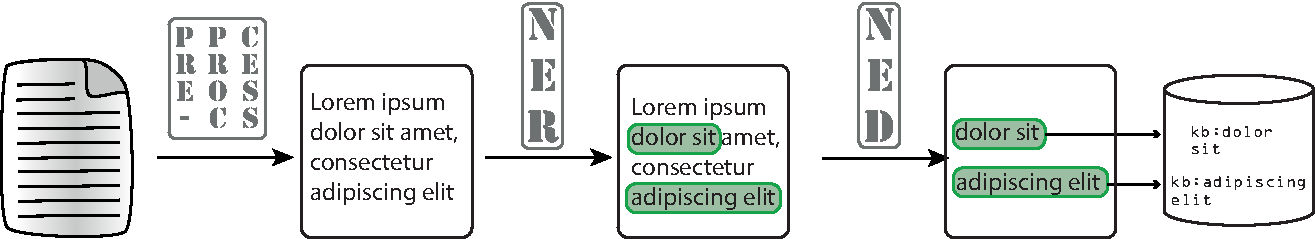
\includegraphics[width=.9\textwidth]{pipeline}

\caption{Overview of the NERD pipeline {\color{red}(provisional)}.}
\label{fig:pipeline}
\end{figure}%

\begin{comment}
Once we have pre-processed the original input text, we use the result as input for the ER component. This component has two main goals that carries out sequentially: first, it detects which words or expressions are able to represent one or more entities in that text. This expressions are usually called \emph{mentions}. This is not a trivial operation: some words may or may not be a mention depending on the surrounding text, as we will see later; and it can be some mentions that our system cannot be able to recognise as such. After this step, a generic NER module should be able to gather a list of candidate entities from the knowledge base for each one of the detected mentions.
\end{comment}

Once we have pre-processed the original input text, we use the result as input for the ER component. This component should find all the entities that are present in the text. These \emph{mentions} can be explicit or implicit, being the first case the most frequent in the state of art, although there are some works that are specialized in the latter one, like \cite{perera2016}. A general approach is the partial or exact match of a sequence of words with an entry in the surface form dictionary. 

Every entity can be called with one or more names; we call each one of these names a \emph{surface form} of a certain entity. As well as one entity can have many surface forms, the same surface form can be used for naming many entities (remember our initial example, where \textit{Born to Run} can be both the album and the song). A surface form dictionary gather all the known surface forms for each entity that is described in the used knowledge base, and relates the former with the latter. They are also known as mention dictionaries.

The desired output of the ER phase is a list of words or phrases that may represent an entity in the text, although we do not know which entities are referred to in it.

\begin{defi}[{\bf Entity}]
An entity is an element from reality that can be called using a name, proper or not, and has a set of properties that describes and characterizes it. People, places, concepts and anything are examples of usual entities. The set of characteristics that describes an entity depends on the needs of each NERD system.
\end{defi}

\begin{defi}[{\bf Mention}]
A mention is a word or phrase in a text that may represent an entity in a natural language text. The mention text should match partially or exactly one of the surface forms that can be recognized by our NER system, or be a pronoun that replaces an entity already mentioned in the text. 
\end{defi}

\begin{defi}[{\bf Surface form}]
A surface form is a possible name (word or phrase) that can be used to refer to an entity in a text. Usually there is many alternative names for the same entity, whilst one of them stands as the \emph{canonical name}, e.g. the most probable one or the one used as title in the corresponding article in Wikipedia. First names and surnames, alias or alternative forms are frequent examples of surface forms.
\end{defi}

The last step in our pipeline is the disambiguation. This occurs in two phases: first, we need to gather the entities that can be represented by each of the mentions provided by the ER component. Second, we need to choose the best candidate in the set of candidate entities for each one of the mentions. 

In the first step, we use the surface form dictionary. This way, we are able to get a set of candidate entities for each identified mention. In case of finding two or more candidate entities for at least one mention in the text, it is needed a disambiguation phase to determine which of the candidate entities fits best as the represented entity by the ambiguous mention. If every mention has exactly one possible entity to correspond with, the annotation is immediate.

If there are many entities that can be assigned to a mention, the disambiguation component must decide which may be the most appropriate. The proposed solutions to this problem are varied, and are the main focus of our paper. In subsequent sections, we delve in the most common approaches and techniques that are used to identify the candidate entity that best fit as the correct annotation for each mention.

The output of a standard ERD pipeline is a list of mentions and their linked entities, frequently embedding the results in the original text by replacing the mentions with hyperlinks. Some additional information can be provided to improve the significance of this result, like lists of candidates, the value of the factor used to decide the best candidate, etcetera.

\medskip

An optional task that is performed in some proposals consists on a final clustering of all mentions that could not be linked with any resource. This let us gather all the similar mentions of this kind across the whole input text, or in a document corpora that is being processed. A general solution is tagging these entities with an empty or null resource. Later we will delve into the implications of this kind of resource.

\bigskip

\noindent\textbf{ERD Challenges}~

The ERD process has many characteristic difficulties that are widely described in all the related bibliography. The most important three ones are listed in \cite{rao2013}, to which we add a fourth: false mentions. Below we briefly describe each one of the problems that we have to face when trying to recognize and disambiguate the entities in a text:

\paragraph{False mentions} As we pointed before, a word or phrase can be or not a mention depending on multiple factors: its grammatical category, its surrounding context, the desired domain for the ERD system (which can bring some semantic idiosyncrasy to the recognition problem), and so on. An accurate ER system must take into account these and other factors to do its task, so it can provide accurate and relevant results to the ED system.

\paragraph{Name variation} One of the main problems in the ER step of the process is related to synonymy. Although any entity can have a conveyed canonical name (which is important to identify it in a computational way), it can also have one or more alternative forms in which it can appear in a text. It can happen in two manners: the explicit way, in which there exists another name for the entity (e.g. Bruce Springsteen and \emph{The Boss}), and the implicit way, where the entity is implicit in a word or phrase that is not just an alternative name, like when we use a pronoun or a more generic denomination to identify an specific object of a class (e.g. ``the Springsteen's album of 1975'' instead of \textit{Born to Run}).

First case is easier to tackle: the number of possible denominations for an entity is limited, so having a complete and up to date knowledge base should be enough to recognize all of the possible manifestations of each entity. This would let us to know about every surface form that should be recognized by our system. The second one requires a more complex processing by inferring the semantics behind the text: to correctly detect the ``Springsteen's album of 1975'' as a mention to \textit{Born to Run}, a system should know about previous mentions in the text to an entity that fits that description. This action would require that the system could be able to recognize, understand and check the semantic relations between entities.

\paragraph{Mention ambiguity} This is the complementary problem of the previous one: the same word or phrase can be used to call two or more entities, which is the fact that motivates the need of disambiguation. Following our working example, we can see this phenomenon with the mention \textit{Born to Run}, as it may refer to both the album, the song or even the recent autobiographical book by Springsteen. However, not having any ambiguity in a text is not always good news, as it can be an indicative of a lack of information in our knowledge base. 

\paragraph{Entity absence} This problem sums up the two previous problems, and can motivate both of them. If we do not have information about a certain entity, we can not determine which surface forms can represent it in a text, therefore we will not be able to recognise them in a text and it will not be considered during the disambiguation phase.

The main reasons for a possible lack of information are three: having selected a bad source for building the knowledge base, having used wrong procedures to extract the information from that source, or working with an obsolete (thus, not up to date with the new information that is generated every day) knowledge base.



\subsection{Fundamentals of Natural Language Processing.}

The pre-processing of an input text makes use of some common NLP techniques, which are discussed below. 

\paragraph{Text Tokenization}
The first step is to modify the structure of the input text to ease the automatic process of it. Generally, text tokenization (or text segmentation) consists on divide the text in more manageable units, like words or sentences. We will focus in the concept of token as words, as it is more useful to ERD than just sentences.

At a first glance, this can seem an easy task, but it is not. Words are not only separated by blank spaces; instead, we can use a plethora of punctuation symbols like dots, commas and more. There are some idiosyncratic aspects that must be faced depending on the language used for writing a text; e.g. in English we have the saxon genitive, in Arabic there are not blank spaces...

Each of these peculiarities must be tackled by defining specific rules to improve the performance over a system that applies only a set of generic rules. The output of this process provides a more manageable set of elements to work with, as it let us to detect possible mentions between these tokens, or to build different combinations of those to be able to recognize multi-word mentions.

\paragraph{Stopword Removal}
One thing that we must take into account in NERD process is the computational cost of it. One good idea could be to reduce the total number of elements that we use as input for the NERD pipeline. To accomplish this, we can exploit the fact that, in every text, there are some words that have no own sense, and they are used instead to make consistent that text. Additionally, there is a large portion of words that cannot be (or it is unlikely enough to ignore them) a mention, so they can be removed from the input to the entity recognition module.

This way, we can prune prepositions, determinants, conjunctions, and so on. We must be careful, though: some stop words can be part of an entities name, e.g. the particle \emph{to} in the album title \textit{Born to Run}, so deleting them might not be that safe and can lead to poor entity recognition performance. For this reason, this operation is more frequent in other areas, such as information retrieval, and is not implemented as part of the NERD pipeline.

\paragraph{POS Tagging}
The Part-of-Speech tagging is one of the most useful operations in the pre-processing step. What it does is to process an input text, detecting and labeling words or a set of words with their grammatical category. It can be done in two ways: by tagging each word as noun, verb, adjective, etcetera; or by identifying the function of each phrasal element, like noun or pronoun phrase, verbal phrase, and so on.

The difficulty of this operation are those words or phrases whose category may be ambiguous, e.g. some words can be identified as verbs or nouns depending on the surrounding context. A correct POS Tagging is very important for NERD, as long as many systems can ignore all words that are not a noun or pronoun to reduce the required computation load, memory usage and general complexity. If a system puts a wrong label, an important mention to an entity could remain hidden to our NERD system.

\paragraph{Stemming}
The stemming is not a common operation in ERD, being more useful in terms of information retrieval, but it follows the mentioned principle of standardize the input to ease its processing. This task consists on replacing each word that is derived from a root form (for instance, conjugated verbs or plural forms of nouns) with that root form. This way we reduce the complexity of the text by limiting the elements which a text can be constructed with.

\subsection{Named Entities.}

Traditionally, the works in ERD has been focused in what has been called \emph{named entities}. Traditionally, this fact motivated the use of the name NERD instead of ERD, which stands for Named Entity Recognition and Disambiguation. Named entities are all those elements from reality that can be identified in an univocal manner with a proper name. The elements that fulfil this definition can generally be distributed en three categories: Person, Location and Organizations. Some authors extends this classification with a fourth class, Miscellaneous, or even a fifth, Events (as proposed in YAGO \cite{yago2007}).

Seminal works in this area considered only entities of this kind, but later, and thanks to the influence of Wikipedia (which has an encyclopedic nature, thus not restricted to only named entities), more and more proposals extended his functionality to what has been called \emph{conceptual entities}, or just entities. This denomination refers to every element in reality that can be named, like concepts, emotions, historical periods... This evolution brings a higher complexity of the process, but greatly increases the functionality of the classic NERD systems. At this point, we consider that the ERD denomination may be more accurate, instead of keep using the NERD name, as it does not limit to the named entities any more.

The chosen approach often depends on the objective of the ERD system: for instance, the first approach is better for a system that is used for automatically enrich news articles, where the relevant entities are people that take part in events that occur in a specific place. On the other hand, a system oriented to verify the correctness of the links between a set of Wikipedia articles could use a broader concept of entity.

\begin{defi}[{\bf Named Entity}]
Named entities are those that are called with proper names, that is, they are unique and recognizable only as themselves. In general, named entities refers to people, organizations and places, although some authors extends this concept to events.
\end{defi}

\begin{defi}[{\bf Conceptual Entity}]
	Conceptual entities are those that are not called with proper names, and they are not unique. Usually, this kind of entities describe concepts, abstract elements or classes, e.g. happiness, art or a lion, respectively.
\end{defi}

\begin{defi}[{\bf Resource}]
A resource is the formal representation of an entity in a information system. It contains all of the relevant (from a NERD point of view) information that can be gathered about that particular entity.
\end{defi}

Below we discuss the two key operations in what concerns to named entities' processing, which we already introduced in the previous subsection.

%% Conceptual Entities

\paragraph{Entity Recognition (ER)}

As described before, mentions can be both implicit or explicit. As the latter is the predominant situation in the state of the art, we will put the focus on it. Our first goal must be to recognise all the mentions that are present in the input text. Once we have processed the raw text and extracted the relevant tokens it contains, the challenge is to determine which of them can represent an entity in that text.

Most systems implement the mention detection by building a set of possible mentions using the token set and querying a surface form dictionary, which we introduced before. This dictionary is the element that contains both every surface form that can be recognized by the system and which entities can represent that surface form, in a similar manner to when we consult a lexicographic dictionary to verify if a word exists.

This step is tricky because mentions can be formed by a variable number of words, and some of these phrases can be contained in another, or overlap between them. A common approach is to extract all the N-grams from a text, that is, all the subsets of up to N adjacent words or tokens. Then, we search in the set of N-grams all the possible mentions. This process is often called ``extraction of N-grams'' from the input text. It can be implemented through a sliding window with fixed length (usually 5 or less) which in each iteration of the process it progressively diminishes its length to extract all the subsets with lower dimension than the given value \textit{n}.

There are a couple of aspects that are worth to take into account in this step. First, we have to take care about the total number of elements that have to be considered, in particular when it comes to set the value of \textit{n}: a value that is too little can leave out some relevant results, or some important information that is vital for a correct disambiguation. We have a good example with the live album by Bruce Springsteen, \textit{Hammersmith Odeon London '75}, which can be easily confused with the theatre where it took place, called Hammersmith Apollo, or the Frank Zappa's live album called just \textit{Hammersmith Odeon}. On the other hand, a value that is too high will lead to a huge amount of mention candidates that have to be queried to the dictionary, looked for candidate entities and, if necessary, disambiguated. A balanced value should be in the range of 4-6 words, according to the bibliography.

Another fact that we have to tackle is overlapping: by using a sliding window in the said way, we may generate some candidates that are also present inside of another possible mention; a good example is the previous one, where the candidate mention ``Hammersmith Odeon'' is contained in other, ``Hammersmith Odeon London '75''. The usual criterion is to discard the first kind of mentions in favour of the longer ones, given that they provide a higher amount of information as they are more specific.

Other methods to locate the mentions in a text are based on simple rules that make use of the POS Tagging information (for example, by gathering all the subjects of each sentence or all the noun phrases), or relying on Machine Learning to accomplish this task. We will talk about Machine Learning applied to ERD in the \autoref{sec:scoreCalculation}.

\begin{defi}[{\bf Candidate Entity}]
	The candidate entities for a mention are those entities in the knowledge base that have a surface form that coincides totally or partially with that mention; i.e. all the entities that may be represented by the said mention in the input text.
\end{defi}

Some authors introduce at this point an additional task known as entity typing \cite{plu2015hybrid}. It consists on determining a type or class for each mention accordingly to a often simple ontology. This information can be used as a preliminary filter to refine the relevance of the elements used as input, but it requires additional information to be successful.

\paragraph{Entity Disambiguation (ED)}  

The Entity Disambiguation task is also referred as Entity Linking in the current state of the art. This comes from the fact that the objective is to link each mention (i.e. a textual representation of an entity) with the resource in the used knowledge base that describes it. This process is often known as \emph{annotation}. However, the resource that must be used to annotate a mention is not always clear: after the ER phase we can have multiple candidate entities for annotating one mention. In these cases, we need to perform a disambiguation step.

\begin{defi}[{\bf Annotation.}]
	Annotation is the task of linking every mention in a text with the resource that describes the entity that is being mentioned. Usually this is done by creating an hyperlink whose text (or anchor) is the mention found in the text, and the destination URL is the URI of the resource that describes the correct entity.
\end{defi}

Once we have a list of mentions after the ER step, the same surface form dictionary can provide the information about which are the candidate entities for each of the recognized mentions. We use each mention provided by the ER component to query the dictionary, given that every mention should match partially or exactly with one surface form in the dictionary. For each mention, we should get a set of candidate entities, that is, entities that can be represented by each surface form. This set can contain zero, one or more elements, which will determine the later actions of the system. This fact lead us to three different scenarios when a mention is being processed:

\begin{enumerate}
\item The mention has only one candidate entity: In this case, we can say that there is no ambiguity and the annotation is immediate. However, this does not mean that this annotation is correct; as we saw above, we are limited by the information that we count with in our knowledge base.
\item The mention has two or more candidate entities: Here we need to decide which of the options is the best for annotating the mention, i.e. we need to \emph{disambiguate} the sense of that mention. To this end we need to establish a disambiguation algorithm, which can be  very simple (e.g. to use most probable sense based in its prior probability) or much more complex (e.g. graphical algorithms or Machine Learning).
\item The mention doesn't have any candidate entities: There are some approaches to tackle this situation. In the beginning, it could lead to discard that mention, as we do not have useful information to process it. Later, it became a common practice to treat this kind of mentions in a particular way: to annotate them with an artificial resource that contains no information, known as NIL, NULL or VOID resource (it would act as a \texttt{null} in a lot of programming languages). This way it can be used to discover information faults in our knowledge base, or to easily detect what has been called as \emph{emerging entities} \cite{hoffart2015}.
\end{enumerate}

In cases 1 and 3, a disambiguation phase is not really necessary -- there is no ambiguity to resolve. However, if there is at least one ambiguous mention in the input text, we must be able to solve this problem by implementing a disambiguation algorithm.

\begin{defi}[{\bf NIL Resource.}]
The NIL resource is an artificial resource introduced by some authors in their NERD systems to be assigned to those mentions that do not get any candidate entities during the NER process. This fact can be used to detect new entities that are not included in the used knowledge base, as they are recognized as mentions but they can not be linked to an entity.
\end{defi}

\begin{defi}[{\bf Prior Frequence Measures.}]
We distinguish two main frequency measures, both of which are independent of the document or corpus of documents that are used as input for the NERD process:
%
\begin{itemize}
\item Prior Probability: It measures the frequency with which a given surface form represents a particular entity. It usually has a normalized value in [0,1], and the sum of the prior probability values from all of the candidate entities tor this mention should be equal to 1 following the concept of probability. In a more formal way: $p_{prob} = P(entity|sf)$.

However, in some works it is used as an absolute value (e.g. the number of times the surface form is used to refer to that entity within a certain corpus of documents). In these cases, we call it just as Prior Frequence.

\item Entity Prior: This value expresses the probability of a given entity to be represented by each of its surface forms. It is usually a normalized value too. In a more formal way: $p_{entity} = P(sf|entity)$.
\end{itemize}
\end{defi}

There are many possible approaches to face the disambiguation problem, as it has been the main challenge that has forced ERD to evolve. First proposals used simple strategies, like picking the most probable candidate entity that may correspond to a detected mention. However, this approach introduces a big margin of error and shows unable to correctly process rare or less frequent entities.

Later systems introduced additional parameters into the decision making process, like using the surrounding context of the mention to support the choice between multiple candidate entities. This requires to have some contextual information about each entity, but it offers a much better result and is able to correctly annotate mentions that refer to an entity other than the most probable one. However, this could not work when trying to distinguish between entities that appear in similar contexts (see our \emph{Hammersmith Odeon} example).

Some authors went one step further and tried to exploit the semantic relations between the entities to determine which of them are more relevant to an input text. This way, if we recognize the entity \emph{Bruce Springsteen}, we can say that the mention \emph{Hammersmith Odeon} is more likely to correspond to the Springsteen's album than the Frank Zappa's, as there exists a semantic relation between the album and the artist who created it. The idea is to discover the combination of candidate entities that maximizes the degree of semantic relation between them. This approach came along the introduction of graphs in the disambiguation algorithms.

After the disambiguation process, the system may do an additional task known as \textit{coreference resolution} \cite{rao2013}. It is highly probable that there are multiple mentions to the same entity in a text, even if different surface forms are used to name it. Coreference resolution consists on clustering the mentions that refer to a same entity and identifying it as a unique mention. This task may be useful to find additional surface forms, as it might determine that a mention represents an entity even if it does not have the mention as a surface form.

We will delve into the different approaches in the \autoref{sec:approximations}, as there are some additional factors that have to be considered during the ERD process.



\subsection{Knowledge Bases}
\label{sec:knowledgeBases}

Almost every ERD system needs an underlying knowledge base to work -- there are some exceptions, but they are a minority and we can consider the knowledge bases as fundamental pieces of the ERD pipeline. Knowledge bases play many roles in the ERD process, as they provide us with lists of entities and surface forms, statistical information about each of them, contextual information to be used during the disambiguation step... Below we enumerate the most frequent knowledge bases in the state of the art, while describing how they can contribute to the ERD goals.

It is worth to note that most of the ERD systems do not utilize these knowledge bases directly. Instead, they use them to build more specific and manageable resources like the already mentioned entity catalogue and surface form dictionary. The pipeline of each system dictates the information that must be extracted from the knowledge base and the way it is structured within that system.

\subsubsection{Wikipedia}~

Wikipedia is one of the most successful projects of its kind. It started as an online encyclopedia in 2001, and since then it has developed a broad variety of ``sister projects'' related to the open data movement. The content in this encyclopedia is community driven, that is, everyone can add or edit content, so it has the potential of being constantly updated and corrected. At the moment of publication of this paper, Wikipedia offers a huge amount of information along its $44.5$ millions pages in 295 languages.

Wikipedia is organized as a traditional encyclopedia in which each entity has an entry in form of an article. These articles do not have a fixed structure, although there are many recommendations and good practices guides to try and standardize the way the information is represented in them. Also, most of the information contained in Wikipedia is human-oriented, that is, it is written in natural language. This makes Wikipedia a great source of data, but hardly usable by automatic means.

In general, each article owns many basic elements, which we outline below:

\begin{itemize}
\item 
Article title: Every article must have an unique title that identifies and briefly describes it. In case of having more than one entity that could be named by the exact same string, they may be differentiated by adding some disambiguation information to the title as a label. This label become part of the title, and it should appear in parentheses. Using our example, the entities that could be named by the string ``Born to Run'' are described in Wikipedia with two articles: ``Born to Run'' for the album, and ``Born to Run (Bruce Springsteen song)'' for the homonym song.

This element can be used as the main surface form or canonical name used to refer to each entity in the knowledge base -- we can assume that it is the most correct and widely accepted form of naming based on the ``community consensus'' of the editors of Wikipedia.

\item Infoboxes: Infoboxes contain part of the most relevant data of the article in form of key-value pairs. The fields that form an infobox are not standardized in a matter of which fields are included or how they should be structured (measure units, reference systems, etc), but there exists many recommended templates that an editor could follow to build the infoboxes in the articles he works on.

\begin{figure}[!ht]
	\centering
	
\includegraphics[width=.3\textwidth]{infoboxExample}
	
	\caption{Example of infobox.}
	\label{fig:infoboxExample}
\end{figure}

Infoboxes constitute the little structured information provided directly by Wikipedia. They can be used to gather diverse properties about an entity to build some contextual information for it, or to stablish named relations with other entities by leveraging the hyperlinks included in its values.

\item Introduction paragraph: In the head of an article there should be a brief text that summarizes the contents of the article. Part of this information is redundant with the included in the infoboxes; however, here it is shown as a natural language text, so it can be very useful for context comparison purposes.

\item Wikilinks: The so called \emph{wikilinks} are hyperlinks that editors of Wikipedia use to link an article with all the related articles. Although these links can appear in many places along the article (like in the infoboxes or in the references at the foot), the main source of wikilinks are the head and the body of the article. The predominant criteria is to insert a hyperlink the first time an entity with a corresponding article is mentioned, leaving the rest of mentions as plain text. An example can be seen in the article of \textit{Born to Run} (see \autoref{fig:wikilinksExample}), where there is a hyperlink to the ``Bruce Springsteen'' article the first time he is mentioned, but not the second time.

\begin{figure}[!ht]
\centering
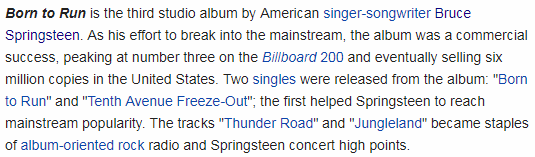
\includegraphics[width=.6\textwidth]{wikilinksExample}

\caption{Example of wikilinks (highlighted words in blue).}
\label{fig:wikilinksExample}
\end{figure}%

Wikilinks are a relevant source of surface forms. Although every article has an unique identifier -- its title --, the hyperlinks may not use that exact title as their anchor text, and put an alias instead. However, wikilinks are particularly useful to discover the relations between two entities. Many ERD systems leverage this feature, most of them following \cite{witten2008}. This work proposes a low-cost semantic relatedness measure, based in the incoming and outgoing links in common between two Wikipedia articles. We discuss this measure later in \autoref{sec:techniques}.

\item References: Following the ``No original research'' principle of Wikipedia%
\footnote{Source: \url{https://en.wikipedia.org/wiki/Wikipedia:No_original_research}}%
, each article should have a list of references that support the information in it. These references appear in the body of the text as citations, so the user can check them right after reading a fact. Although not very often utilized by ERD systems, references could provide them with valuable contextual information by consulting these sources, or just by using their titles and authors.

\item Categories list: Wikipedia has a broad structure of semantic categories, which groups articles in classes like ``1975 albums'' or ``Bruce Springsteen albums''. There exists parenting relations between categories, and they are not restricted: a category can have multiple parents and children. However, the resulting structure is not a tree, and does not define a coherent and exhaustive hierarchy. It forms a somewhat chaotic directed graph where categories act more as semantic tags than as semantic classes from an exhaustive ontology.

They may be useful for the ERD process, though. They might let us determine the topics of a text based on the entities that make its appearance in it and the categories they belong to, and can also serve as key terms in the contextual information of an entity.

\end{itemize}

Also, we can differentiate between four types of pages in Wikipedia:

\begin{itemize}
	
\item Articles: These are the standard documents that contains the previously exposed elements. Using the articles, we can build the entity catalogue, and also the surface form dictionary by leveraging the wikilinks in them. Those systems that make use of graphs to model the information can use the wikilinks to stablish relations between the entities.

\item Redirection pages: The redirection pages are empty articles that only contains a title and a hyperlink to another article. This pages are placeholders for the aliases of an entity that differ from its canonical representation, so the user could be redirected to the correct article even if the search string does not match exactly with the article title. 

For instance, the search term ``Springsteen'' leads to an empty document, whose title is exactly ``Springsteen'', that automatically redirects to the main article, ``Bruce Springsteen''. This pages are mainly used to gather the most frequent aliases that are used to refer to each entity, so they can be used to enrich the surface form dictionary.

\item Disambiguation pages: Disambiguation pages contain a list of hyperlinks to all the articles that could be the correct match for a given search string. These pages are needed when the same name or phrase can represent many entities, so they can be useful to stablish new relations between entities and surface forms. For instance, if we search ``Born to Run'' we will be redirected to a disambiguation page that contains a list of links with up to fourteen articles.

\item List pages: These documents put together links to multiple articles that belongs to a specific semantic group. This pages does not respond to the categories classification, nor other similar structure, although they play a similar role. For instance, many albums by Bruce Springsteen are included in the list ``List of rock albums'', while the category ``Rock albums'' does not exist.

\end{itemize}

Wikipedia was the first knowledge base used for ERD purposes, and it is still one of the most common ones as it is open, very rich, and very adequate for NLP analysis as long as most information in it is written natural language. This helps the systems that leverage contextual information to compare the habitual context of an entity with the context of a mention in the input text.

However, the lack of a fixed structure may not be optimal for many systems, so they opt for more structured and consistent knowledge bases, like DBpedia or YAGO (which are ultimately based on Wikipedia, as we will see). We deal with these alternatives in the following paragraphs.

\subsubsection{DBpedia}~

DBpedia (2007) is one of the most successful projects whose aim is to extract the knowledge in Wikipedia and give it a defined structure. DBpedia storages this information in RDF, so the search mechanisms are not restricted to term matching as in Wikipedia. Instead, it lets an user to formulate expressive queries which greatly improves the versatility and usability by automatic means of this knowledge base. The foundation of this structure is the DBpedia ontology, which consists on a hierarchy of 685 semantic classes, each one with its own properties that describe it.

Over the years, the ontology has evolved from a tree into a graph, where each class can have more than one parent. This increases the richness and flexibility of the ontology in a general domain environment. Each entity, named as a \emph{resource}, is given an unique name --in general, its title in Wikipedia without the trailing parenthesis--, and a potentially huge set of properties. These properties describe the entity in a form of key-value pairs, but in a more standardized fashion that Wikipedia's infoboxes: properties are also resources that have its own properties too, so everything in DBpedia is grounded accordingly to a defined criteria. 

However, Wikipedia has a vast amount of information that is human-oriented and hence expressed in natural language, so it is hard to automatically translate it to the DBpedia's structure. Instead, DBpedia relies on the portion of structured and semi-structured information that exists in Wikipedia:
%
\begin{itemize}
\item Infoboxes are the main source of structured information. They contain the main facts of the entity that is described in an article, as well as a set of links that connects that entity with others. However, the variability in infoboxes' structure requires a combination of techniques to correctly extract its information, which include templates, type recognition for the data, etcetera.
\item Wikipedia categories, although somewhat chaotic and unstructured, are useful to classify the entities into the DBpedia ontology. To this end, a mapping between the category graph and the DBpedia ontology must be created and constantly updated.
\item Disambiguation and redirection pages provide with aliases of the entities, which are stored as \emph{lexicalizations}. This concept is also key for the multi-lingual support of DBpedia.
\item Links to versions in another languages, which let DBpedia to connect resources between its different versions.
\end{itemize}

Along its development, DBpedia has grown as an invaluable source of structured knowledge, as it offers many features that can be used in multiple environments. For ERD, the advantages are clear: it provides a large and up-to-date entity repository, thanks to its almost real-time update module against Wikipedia; it contains a detailed dictionary of surface forms and context samples for each entity, as well as a rich semantic network between them, which let us utilize it for all the steps in ERD.

\subsubsection{YAGO}~

YAGO \cite{yago2007,yago2013,yago2015} combines the rich semantic knowledge of Wikipedia with the highly detailed taxonomy of Wordnet. From the first, YAGO takes a list of entities, category information, relations between entities (based on wikilinks), most of the surface forms and contextual information. From the latter, YAGO adopts its taxonomy, which it fills with the entities from Wikipedia by applying a mapping between Wikipedia categories and Wordnet synsets. All of this information is stored as RDFS triples, following an SPO model (Subject, Predicate, Object), an later SPOTL, a customised version of the previous one that also includes Time and Localizations and is introduced in YAGO2. In YAGO, relations or predicates are also considered entities, so it is possible to create relations between relations, as well as assigning properties to a relation.

In YAGO, each entity is identified with an unique string, which is used as the subject in all RDF triples this entity is present. Each triple is called a \emph{fact}, being each fact assigned an unique identifier. Facts are also entities -- thus, they can participate in new triples following the notion of \emph{reification}.

Entities are assigned to different classes from the WordNet taxonomy by using the \texttt{type} relation. Classes are entities that belong to the \texttt{Class} class, and they relate to each other through the \texttt{subClassOf} relation, giving this taxonomy a hierarchical structure following the one that exists between the Wordnet \emph{synsets}.

YAGO was updated in 2013 and 2015 to its versions 2 and 3, respectively. These new versions expand the scope of YAGO. YAGO2 \cite{yago2013} adds support to spatial and temporal dimensions by introducing specific relations to link entities and literals. These relations may describe the start or end in time that is proper of some entity types, as well as the place where an event occurs or an entity is placed. To allow this expansion, they add Geonames and Universal WordNet to its knowledge sources. This version also revises the structure of YAGO to improve its extensibility. Remaining new features consists on improving the amount of information that is extracted from Wikipedia, creating specific relations to include anchor texts from wikilinks, Wikipedia categories and citation data, as well as the abstract paragraph from each articles to use it as context for the entity. Later, YAGO3 \cite{yago2013} improves the multi-language support of YAGO by leveraging the information in Wikidata and the different versions of Wikipedia. The original YAGO2 is expanded with the information in languages other than English.

\subsubsection{Freebase}~

Freebase \cite{bollacker2007,bollacker2008} is a currently extinguished project whose aim was to replicate the Wikipedia project in a more structured fashion. That is, a collaborative, community-driven knowledge base that conciliates the information gathered from multiple unstructured sources. In contrast with YAGO, which can be considered a similar initiative, Freebase would be maintained by its community -- that is, open, and not proprietary as YAGO is--, and having a more flexible taxonomy to manage its entities. Freebase was acquired by Google in 2010 and later closed and discontinued in 2015. Today, Freebase is integrated in Google's Knowledge Graph%
\footnote{https://www.google.com/intl/bn/insidesearch/features/search/knowledge.html}%
\footnote{https://developers.google.com/knowledge-graph}%
.

Freebase proposed a graphical representation of the knowledge, built with many elements. Entities are called \emph{topics}, and have an unique identifier. Relations between entities are called \emph{properties}, as well as the relation between an entity and a literal (e.g. time stamp, numeric value, etcetera). Entities belong to one or many \emph{types}, the equivalent to Wikipedia categories, although there does not exist any hierarchy or parenting relation between these types. However, they are also entities themselves, so they can be described though properties and relate with other nodes in the graph. To allow guiding the way an entity is described, there exists \emph{schemas}, or sets of obligatory properties for an entity depending on its type or types.

\subsubsection{Wikidata}~

Wikidata was started in 2012 by the Wikipedia Foundation. This knowledge base aims to provide information and multimedia data that is adequate for both human and automatic processing. It also serves as a hub for all the structured information in its sister projects, being the main one Wikipedia. Wikidata follows the same principles than its sister proyects: it is free and open, and it promotes a collaborative philosophy for the creation and update of its contents. Wikidata also tries its best to consolidate the multilingual information, collecting and storing all the information in as many languages as it can.

Entities are represented as \emph{items} in Wikidata. Each item has an unique identifier: a numeric code to be used by machines, as well as its own page where all its related information is shown. Ever item is also assigned one or more \emph{labels}, a more meaningful name that is more suitable for human consumption.  However, this label may not be unique; it is only for clarification purposes. Items have two more basic features: \emph{descriptions}, which are brief definitions of the depicted entity, and \emph{aliases}, that are lists of surface forms that can be used to refer to the entity. Labels, descriptions and aliases are language-specific and are separated by its language.

Items also have \emph{statements}, the relations that complete the semantics of an entity. These relations can be established between entities, in a similar fashion to other knowledge bases' structure, but also between an item and a number or a literal. Statements store varied information about an entity, which includes semantic classes, dates, places, and so on. Statements in Wikidata are items themselves, which allows them to be characterized with their own labels, descriptions and aliases, although they can not be enriched with sentences and are stored in their own name space.

Wikidata keeps the ``secondary knowledge source'' vocation that had Wikipedia, so every fact that is stored in it must have an explicit source. These sources are gathered in each item's page as a list of hyperlinks.

\subsubsection{BabelNet}~

BabelNet \cite{navigli2010,navigli2012} is an online encyclopaedia and semantic network that started in 2010. Similarly to YAGO, it takes Wikipedia (instead of DBpedia) and WordNet and merges them in an unique knowledge base. However, the amount of used information sources has been increasing along its new versions, including knowledge bases like Wikidata, Geonames or Wiktionary among others.

In contrast with YAGO, BabelNet implements a graph structure, where entities are represented as nodes and semantic relations between pairs of entities are represented as directed, labelled edges. These relations describe the semantics that somewhat links two entities. However, they are not arbitrary, as BabelNet defines a fixed set of relations that can be used. Relations are extracted from both WordNet, specifically its semantic pointers between its \emph{synsets} or sets of synonyms, and Wikipedia, by leveraging its wikilinks structure. Relationships are unified by mapping WordNet and Wikipedia entries.

Special relationships are created between all entities that belong to a WordNet's synset (for instance, synonymy or hypernymy/generalization and hyponymy/specialization), which allows BabelNet to create contextual information for each concept, as similar (i.e. related) concepts tend to appear altogether and thus they constitute a representative context for comparison purposes.

Entities have an unique identifier in English coming from WordNet and the English Wikipedia, although each entity node also contains a set of \emph{lexicalizations}. Lexicalizations are special surface forms that refer to the name of the entity in a different language than English. This way, multilingual information is easily accessible and unified against the English entity catalogue. The set of lexicalizations of an entity is called its \emph{babel synset}. Each entity also counts with one or more glosses in different languages that comes from the definition that every synset in Wordnet has, or the first sentence of the corresponding Wikipedia article.

\subsubsection{More...}~

Below we briefly describe some knowledge bases with a much lesser or non-existent presence in the state of the art, as they cover a very limited domain that has not gotten much interest from the scientific community. However, we consider that they may provide a high value when facing a more specific problem than those tackled by most of the systems we describe in this paper, so we include them here for testimonial purposes.

\begin{itemize}
\item WordNet: Is a lexical database in English language. It contains a plethora of nouns, verbs, adjectives and adverbs distributed in sets of synonym words called \emph{synsets}. These synsets act as semantic classes or categories, and they are interconnected through semantic and lexical relations. They have also brief definitions that describe the set of words from a semantic point of view, as well as a set of short sentences to illustrate the use of its elements. Currently, WordNet defines more than $117\,000$ synsets. Between these synsets there can exist many relations, like hyperonymy, or its complement, hyponimy, which exists between a more general synset (e.g. instruments) and a more specific synset (e.g. guitars).
\item Geonames: Is a geographical database that stores more than 10 million geographical localizations. Each localization may be described by its geographic coordinates, one or multiple denominations and secondary data like population, altitude, etcetera. Places are classified in one of up to 9 classes, and can be tagged with up to 645 categories.
\item IMDb: Is probably the biggest user-oriented cinema database. It stores not only movies data, but also about everything surrounding the cinema industry, like professionals, localizations of scenes, professional and user reviews, etcetera.
\item Last.fm: Is a database that is specialized in music industry that gathers information about albums, artists, producers, discographic labels, and so on. It also has a user-oriented functionality that allows people to create lists and reviews that may be useful for entity disambiguation purposes in this specific environment.
\item DBLP: Is a citation and reference database that allows to explore the publications belonging to computer science, as well as provides access to both metadata and electronic editions of the papers it links.
\end{itemize}
















\section{Approximations to ERD.}
\label{sec:approximations}

\hspace*{30pt}
\noindent
\begin{minipage}[b]{.4\textwidth}%
	\schema{
		\schemabox{a. Información}
	}{
		\schemabox{
			Prominencia \\
			Local \\
			Colectivo
		}
	}

	\medskip

	\schema{
		\schemabox{b. Tipo de texto}
	}{
		\schemabox{
			Estándar \\
			\textit{Microposts}
		}
	}
\end{minipage}
%	\medskip
\hspace*{20pt}
\begin{minipage}[b]{.4\textwidth}%
	\schema{
		\schemabox{c. Modelos de datos}
	}{
		\schemabox{
			\textit{Bag of Words} \\
			Grafos
		}
	}

	\medskip

	\schema{
		\schemabox{d. Métodos}
	}{
		\schemabox{
			Matemáticos \\
			\schema{
				\schemabox{Aprendizaje automático}
			}{
				\schemabox{
					Supervisado
					%: Deciden la entidad candidata adecuada en base\\ a un conjunto de entrenamiento totalmente anotado.
					\\
					Semi-supervisado
					%: Deciden la entidad candidata adecuada en base\\ a un conjunto de entrenamiento parcialmente anotado.
					\\
					No supervisado
					%: Deciden la entidad candidata adecuada en base\\ a un conjunto de entrenamiento sin anotar.
				}
			}
		}
	}
\end{minipage}

\subsection{Used Information During the Disambiguation Phase.}

This classification is proposed in \cite{aida2016}.

\paragraph{Prominence-based Methods}

These are the first and most simple approach that has been proposed to solve the ambiguity problem. The idea is to annotate each ambiguous mention with the most probable candidate entity, i.e. that with the higher prior probability.

As we pointed before, this method has an inherent error probability that in many cases is not negligible. Lets assume that for the surface form ``Born to Run'' we only have two candidate entities, the album and the song, with values of prior probability of $0.6$ and $0.4$, respectively (note that these are normalized values). Every time the mention ``Born to Run'' is found, it will be linked with the entity ``Born to Run (music album)''. However, if the probability model is correct in 4 out of 10 times that mention is used in a text it should be referring to the entity ``Born to Run (song)'', so our algorithm is throwing a wrong result the $40\%$ of the times.

The previous situation can be mitigated in very restricted or specialized environments where the domain of senses is limited, so the ambiguity, if exists, presents a very shafted probability distribution, so the error margin that we introduce is low enough to get acceptable results.

This approach assumes that there is frequency information available for each of the surface forms which the system knows about. There are some sources that can be used to this end:

\begin{itemize}
\item Statistical models of the used language: Given the language in which the text has been written, we can use linguistic studies to determine the probability of each possible sense for each of the surface forms. However, this data is generic and may not be fully representative of the application environment, e.g. when working in a restricted domain where the most specialized senses (and probably the more adequate ones) gets low prior probability values in a linguistic model.

Using this models could also require some adaptation to the knowledge base, as they may include surface forms and entities that do not exist in the knowledge base. This is specially true if we have to work with normalized prior probability values.

\item Statistical models of a selected document corpus: We can build a corpus of relevant documents for a better adaptation to the domain of our interest. However, a good enough collection of documents should be large to be reliable, so it requires a higher effort than just using some existing statistical models. Also, we would need to build a new corpus if we change or extend the domain of the problem.

\item Alternative frequency measures: We can make use of other measures to acknowledge the prominence of each entity, like the number of results in search engines. It provides updated information in a very broad domain; however, it is not very reliable as some entities that are prevalent in time might gather a higher number of references that do not accurately represent its real significance. On the other hand, some entities could benefit from a great impact in a short time frame, getting a lot of references although its relevance in the long term would not be great.

\item Wikilinks\footnote{As explained in \autoref{sec:knowledgeBases}, wikilinks are hyperlinks that link pairs of Wikipedia documents with a directed relation. When an entity is mentioned in another entity's article, that mention is annotated with a link to former entity's article.}: This is one of the most used methods, as it is both reliable and accurate. Information within Wikipedia can be considered canonical and truly representative of the reality, as it is continuously updated and revised by a collective of redactors.

The prominence measure is the number of wikilinks that point to the entity's article, assuming that the more linked an entity is, the more prominent it is in the domain depicted by the whole Wikipedia. It also let us limit the domain of the process by using the category hierarchy of Wikipedia.
\end{itemize}

\paragraph{Local Methods}

As pointed before, prominence-based methods always have an error percentage that can not be avoided by any means. Local methods exploits a new and powerful resource: the context of the mention. We can assume that every time we mention a certain entity, it should take place in a similar context. For example, the context of \emph{Born to Run} should always address some music-related topic. It would be strange if we find a mention to \emph{Born to Run} in a text related to Michelangelo or the Renaissance.

The idea behind this approach is to determine which of the candidate entities for a given mention is the most adequate by analysing its context. To this end, we need to describe each entity in our knowledge base with some contextual information. This information can adopt many forms, but we will address it below. This way, we can compare the contextual information of each candidate entity with the context of the mention we want to disambiguate, annotating it with the entity whose context is best represented in the surrounding context of the mention.

We may understand contextual information in two ways:

\begin{itemize}
\item Plain text: The registered context is one or more representative texts where the entity is mentioned. This way, the information can be noisy and it would need to be refined (e.g. stopwords removed) to make the process more accurate and efficient. Wikipedia articles are a good resource to use to this end, as they also contain surface forms corresponding to other entities that are semantically related, providing a rich context in a semantic manner.
\item Keywords: The context consists in a set of words or phrases that are commonly used together with the surface forms of the entity. The sources of this keywords are diverse: most common words (apart from the surface form itself) in a corpus of documents that addresses the entity, lists of semantic tags (e.g. Wikipedia category names), etcetera.
\end{itemize}

Contextual information can be represented in multiple forms that may determine the way it should be compared. The most simple representation is as mere text strings, but most proposals use a vectorial representation of the context. This way, texts are represented as vectors in which each word is a new dimension, so the text is already tokenized and reduced to its fundamental components. This makes easier to compare between contexts by determining the overlapping between vectors, as we already know which components must be considered in this process, instead of having a bunch of words all together.

This methods provide better results that the prominence-based ones, as it takes into account the nature of the text in which the mention has appeared. By contrast, the methods that only use the prominence as decision factor are totally independent of the particular text. However, this approach is not enough when facing texts that lack context, e.g. microposts, or in which the context may not have enough quality. It also finds very difficult disambiguating entities that are tangential to the predominant topics of the text: many systems that only rely on this methods would struggle to correctly annotate a mention to the 1965 Bob Dylan's album, \emph{Highway 61 Revisited}, in a text about the history of this famous North-American road, although it is a feasible mention to be found in that context.

\paragraph{Collective Methods}

{\color{red} ¿Cambiar por \emph{Global}? Así se les llama en algunos trabajos (ver PBOH) y puede ser más coherente.}

We have seen that using only the contextual information in the input text may not be enough to obtain adequate results. This motivates the need of this new approach, that tries to exploit the semantics behind the entities to support the process of disambiguation of ambiguous mentions.

As long as entities are representations of elements of reality, we should be able to stablish relations between them; e.g. every album has been created by an artist, who was born in a city located in a certain country, in which a lot of other significant people was born, and so on. There are many \emph{semantic relations} between entities that can be identified and registered in our knowledge base so we can use it for our benefit.

To this end, it is specially useful a specific model for representing the information: a graph, which we will call \emph{candidate graph}. In this kind of graph, entities would be represented as nodes or vertices, and the relations between them as edges. The strength of the relations can be modelled as a weight for each of the edges, letting us to recognize which relations are stronger than others when having to decide between two candidate entities.

This approach introduces two ways of resolving the ambiguity in a NERD process:

\begin{itemize}
\item Sequential: The ambiguity of the mentions in the input text is solved in a sequential way, although for every mention we look at the candidates of the rest of the ambiguous mentions or even those that are not ambiguous. This way, we can use the unambiguous mentions to determine the best of the candidate entities for each of the ambiguous mentions. The already disambiguated ones could be also used to process the following mentions that present some ambiguity, but it would favour the importance of the first mentions in the text. However, this may be appropriate in some scenarios, like the automatic annotation of news articles.
\item Joint: Another approach is to try to disambiguate all the ambiguous mentions in only one step. This kind of operation is usually very complex, and it requires the use of approximations to be accomplished in a reasonable time. The main objective in this case is discovering which of the possible combination of annotations maximizes the semantic coherence between them. However, when the number of mentions or the ambiguity degree in a text is high, the complexity of the problem could become impossible to handle.
\end{itemize}

{\color{red} Hablar de la fórmula de semejanza de Milne y Witten, ampliamente utilizada en el estado del arte. Referenciar \autoref{sec:techniques:semantic}.}

\subsection{Data Models.}

\paragraph{Bag of Words}

The simplest representation of a relevant part of the information that is necessary for the disambiguation process is the \emph{bag of words}. Proposals that follows this model represent the surface forms, candidate entities and contextual information as arrays or vectors of words.

This is an easy to implement method to store the information, but it lacks usability in many aspects. First, its relation capacity is very limited: in general, we will have a set of entities, where each of them has attached a vector of surface forms. What we save in terms of data representation, it is needed to be done in terms of linking and giving consistence to all the information that has to be managed during the NERD process. It also fails in weighting correctly the influence of the different elements used in the process, as it needs additional structures to include that kind of information into the pipeline.

{\color{red} Hablar de la fórmula de semejanza del coseno como método habitual de cálculo de la semejanza entre dos textos. Referenciar \autoref{sec:techniques:context}.}

\paragraph{Graphs}

The most frequent procedure is as follows: after we model the information in our knowledge base as a (ideally) weighted graph, we extract the sub-graph that includes all the entities that have been identified as candidate entities for any mention in the input text. Based the hypothesis of that, in a text, the predominant topic is coherent and all mentions in the text should relate to that topic, the correct entities in the candidate set should show a high degree of semantic relatedness. Our main objective should be, then, finding the sub-set of candidates that offer the highest total weight.

We face many challenges here:

\begin{itemize}
	\item How to calculate the weights: First, we need to define how the semantic relatedness will be measured. A very used approach is the proposed in \cite{witten2008}: it calculates the semantic similarity between two entities by evaluating the overlapping in the wikilinks in their respective Wikipedia articles. The more links are shared by both articles, the more similar will be their corresponding entities. This measure takes into account both the incident wikilinks (links from other articles) and the references to other articles.
	
	We can define a more complex model in which aspects like distance between nodes have to be taken into account. This would let us to define new weights that could serve to better catch the semantics in a text by including some subtle relations that are not contemplated in a model in which only the directly related nodes are considered.
	
	\item Size of the candidate graph: In general, we might consider that, given that every text has to be topically coherent, every entity should be connected to at least one other entity. However, this is not always true: in many cases, there are some entities that remain isolated in the candidate graph, as they can not be directly related with any other entity in the graph.
	
	To solve this, we can expand the candidate graph to catch subtler relations. For example, we can not only consider candidate nodes, but the adjacent nodes too. Of course, these nodes will not be considered as candidates for annotating the mentions in the input text, but they would be used to calculate the weights of the relations between entities.
	
	However, this can lead to the construction of huge graphs that can not be handled without introducing approximations or using an outstanding hardware to complete the NERD process in an acceptable lapse of time. 
	
	\item Algorithm: As it was pointed before, in some cases the generated graph can not be processed in a straight manner, e.g. computing the weights of every resulting combination, as the number of combinations or the complexity of the calculus is just unmanageable in a finite time.
	
	In this cases it is needed to use approximations that belong to graph theory, like Random Walks or Random Trees. We will talk about them later in \autoref{sec:edSystems}.
\end{itemize}

Taking advantage of the use of graphical models, we can extend it to other parts of the problem; in particular, to model the mentions and the candidate entities that correspond to each one of them. This model was initially proposed in \cite{yosef2011}. We can see a small example in \autoref{fig:fullGraphExample}.

\begin{figure}[!ht]
	\centering
	
	
\includegraphics[width=.3\textwidth]{tbd}
	\caption{Full graph example.}
	\label{fig:fullGraphExample}
\end{figure}

\subsection{Candidate Entity Score Calculation.}
\label{sec:scoreCalculation}

\paragraph{Mathematical Models.}~

Proposals that adopt this kind of approach rely on mathematical expressions to weigh the likeness of each candidate to be the optimal annotation, that is, to score it. A well constructed formula should lead to the most adequate candidate entity getting the highest value.

These formulae are constructed by attending to many measurable parameters for each mention-candidate entity pair. The nature of these factors is varied, but can be summarized in three categories: prominence of the candidate, similarity between a mention and its candidate entities, and semantic coherence between candidate entities. We will delve into this classification later in \autoref{sec:techniques}.

The calculated score can be also used to fine tuning the system. It is possible to impose a minimum distance between the highest ranked candidates to accept the results as valid. For instance, the highest ranked candidate is used as the correct annotation only if it gets a certain amount above the second ranked candidate, i.e. there is a certain degree of confidence in the ranking result. It can also be useful to remove all the candidates that get a score that is below a predefined value, so the non-relevant candidates are not introduced in a subsequent disambiguation step. This is particularly interesting in graphical models, as every candidate that is considered increases the size of the graph, thus increasing the complexity of the disambiguation problem.

\paragraph{Machine Learning.}~

As pointed in \cite{rizzo2011nerd}, machine learning has been introduced in NERD with great success -- since its first systems, there has been a niche of machine learning-oriented proposals, being \cite{milne2008} the first example of this fact. These techniques let a system to be \emph{trained} to recognize, disambiguate or perform both tasks by learning related examples. These can be both correct annotations --positive examples-- or incorrect annotations --negative examples--, although it may be defined by the author or the implemented learning algorithms.

\cite{nadeau2007survey} describe the three common approaches to machine learning:

\smallskip

\hfill
\begin{minipage}{.98\textwidth}
	
\paragraph{Supervised Methods.}

These require an initial corpus of labeled documents, which will provide with examples that will be used by the system as a reference for the decision making. This corpus should be both large and complete, so it provides enough valuable examples to support the annotation generation in diverse scenarios, e.g. different mentions and contexts for the same entity. Some of the most common learning algorithms are briefly depicted in \autoref{sec:techniques:ml}.

These methods present some downsides. First, they may be expensive, as they usually must be manually constructed to provide a solid ground and a high confidence about the information that it contains. However, this fact can be overcome by using an already existent resource to train a system, like Wikipedia \cite{milne2008}. Second, the scope of the training set highly determines the performance of a system, so the quality exigence implies using a carefully designed document corpus. This is particularly relevant when facing restrictive environments with very limited domains, where specialized knowledge may be needed and there may not be enough documents to build an adequate corpus.

\paragraph{Semi-supervised Methods.}

These methods try to overcome the drawbacks of pure supervised methods while keeping their reliability. Semi-supervised approaches only need a small training set, which will be supported by additional information and further expanded by including unlabeled documents. Labeled documents act as the seed for the learning process, which includes the automatic labelling of the unlabeled data to be used as examples by the system. These methods are particularly effective in specialized environments, as they often have very concrete mentions and entities.

\paragraph{Unsupervised Methods.}

These methods rely on the capacity of a system to discover implicit patterns and structures in a corpus of unlabeled documents. By analysing an input set of documents, a machine learning system should be able to infer some rules to help in its decision making.

\end{minipage}



\subsection{Language Treatment.}

As pointed before, NERD process is very language-dependant. This factor can influence, or even determine, how the process have to be implemented, e.g. which algorithms can be applied, which operations should be done...

In consequence, language is something that can not be unseen when designing and implementing a NERD system. There are three possible ways in which this factor can be faced:

\paragraph{Monolingual.}

In general, a NERD system is designed for one language in particular, so it should only provide good results when processing texts in that language. To be able to satisfactorily process texts in other languages, the system itself must change to adapt to the idiosyncrasy of that language. 

That is the reason behind the modular architecture that most of the  NERD systems tend to adopt recently. This way, we can use one or another module depending on the language that must be computed. However, it forces us to implement a new module for each new language that must be recognized by our system.

\paragraph{Multilingual.}

Given that some languages present many similar characteristics, it should be possible to design and implement a tool that could face many languages instead of only one. In this group we would include those systems that are able to detect the language of the input text and automatically process it with the corresponding module (e.g. AGDISTIS \cite{gerbil2015}), even if there are separate modules for each of the compatible languages.

In general, this only applies for the first stages of the process: we can gather many pre-processing operations that are common to a handful of languages. This principle can also work for mention detection by using techniques as capitalization analysis and so on. It does not propagate to further steps, though: both recognition and disambiguation are specific for each language, and these operations need to count on language specific information to be accomplished.

\paragraph{Cross-lingual.}

A novel approach is to try to build a generic system that can process any text in almost any language. A system of this kind would rely on a huge and well-formed knowledge base that owns information of each entity in every compatible language. This approach is motivated by the apparition of rich multilingual knowledge bases, e.g. DBpedia or Wikidata, that provide a solid foundation for the NERD process. This way, there is only one pipeline that is applied to every input text. The only difference will be the information used for recognizing and disambiguating the mentions in it. 

One interesting model is the proposed in x-LiSA \cite{zhang2014}. It consists in selecting one language as ``main language'' (along with its corresponding knowledge base) and using the multilingual information as ``support knowledge bases'', one for each language. The latter would be used to recognize and gather all the candidate entities, as well as their related information (e.g. contextual and statistic information). However, the disambiguation is done using the data from the main knowledge base. The problem is that the contextual information of the entities is in a different language than the text, so some automatic translation is applied to get the context information from the input text.

\subsection{Text Type.}

\paragraph{Standard.}

Apart from the language, the nature of the text can influence heavily on the performance of a system. Traditionally, a good example of a typical input text for the NERD pipeline are news articles. This kind of text contains many entities and counts on some contextual information. It also is well constructed -- that is, it uses proper grammatical structures, a correct punctuation criteria, etcetera. The mentions to entities are, in general, explicit and complete, at least the first time it is included in a text. It is not uncommon to find an entity that is mentioned many times along the input text, e.g. the entity ``Bruce Springsteen'' can be called as ``Bruce Springsteen'' in its first apparition, and just as ``Springsteen'' the following times it is mentioned.

Some systems consider this fact in his NERD pipeline, often using this co-occurrence of many surface forms of a particular entity to increase the probability of that entity being the correct one. Others go another step beyond that and extends this search to pronouns in the text -- i.e. mentions to implicit entities, as it can provide additional information about the genre or number of the entity.

However, the length of the text, thus the richness in contextual information for the disambiguation process, is the key factor that distinguishes the standard type of text from the other main kind of texts, which is explained below.

Within this category we can find those texts whose length would make them unmanageable if we apply certain NERD strategies. If we use a pipeline that simultaneously uses \emph{all} the mention or entities in the input document, e.g. a Joint model or a graphical model, the number of entities is an obvious limiting factor. Given that the longer is a text, the more mentions and entities it will contain, it is needed a workaround for specially long texts that could be used as an input document, e.g. a novel or History book. Even if the scalability factor was not an issue, many proposals would suffer since it would be difficult, if not impossible, to exploit the thematic coherence hypothesis that we enunciated before due to the high number of topics that would be implied in a long text. In some cases, it just would be impossible to determine a restricted domain for the whole text.

Typical strategies to tackle this kind of texts consist on dividing the book in lesser units, e.g. chapters, paragraphs, etcetera. This way, the huge input document is converted into a collection of more manageable documents that can be processed one by one, as they would fit in the concept of \emph{standard texts}, thus being processable by most of the systems in the state of the art. To the best of our knowledge, there are not any systems that are focused on processing this kind of texts, nor any theoretical approach to make it possible without a previous simplification of the input. 

\paragraph{Microposts.}

\emph{Microposts} are one of the latest and bigger challenges for the NERD field of study. Microposts are very short texts that may be poorly constructed. This fact puts a big obstacle to perform NERD on this kind of texts: the lack of context. \emph{Tweets}, the user publications in the Twitter social network, are the best example of microposts: shorter than 140 characters, idiosyncratic structures (\emph{hashtags}, \emph{user mentions}) and an informal style constitutes a huge challenge for traditional NERD systems.

The necessity of processing this kind of texts started precisely with the boom of Twitter. Twitter is a very agile and real-time social network, in which the users can publish public messages in their timelines. The interaction with other users can take three forms, that originate some structures that are peculiar to this social network:

\begin{itemize}
\item User mentions: In general, any user can \emph{mention} any other user in a message by adding ``@username'' to it, where ``username'' is the user name of the mentioned user. This action starts a ``conversation'', that is, a chain of tweets between these two users. It can be broader if any other user is mentioned in the conversation. 

This has an interesting  consequence for NERD: it originates new surface forms, as an entity can be referred to with its user name in Twitter, e.g. @BruceSpringsteen. Note that there can not be blank spaces in a user name. An alternative is cleaning the user mentions by removing the ``@'' symbol and trying to relate the result with a traditional surface form, e.g. by trying to separate the words that form the user name based in its capitalization.

This kind of structure is relevant when facing named entities, as it always refers to an user of Twitter.

\item Hashtags: A \emph{hashtag} is a label with the form ``\#hashtag'' that is used to tag a tweet. A tweet can contain zero, one or more hashtags. They are used to group topically similar tweets, as they usually describes the context in which the tweet is published. With regards to NERD, hashtags may give contextual information about the content of the message, so it may be useful to exploit them.

In this case we face the same problem as with user names, so the solution may be the same: we remove the ``\#'' symbol and we separate the words in the hashtag based on the capitalization of its characters. An example of this may be ``\#BruceSpringsteenLiveConcert'', which would generate ``Bruce Springsteen Live Concert''. This can be useful to disambiguate a mention like ``The Boss'' in the tweet \textit{``He's really The Boss! \#BruceSpringsteenLiveConcert''}, as it provides us a better context than just the non-hashtag text.

\item Retweet: A \emph{retweet} consists on publishing an another user's tweet in our own timeline. It has no effect on the NERD process beyond of getting duplicate messages in an input set of tweets.
\end{itemize}

Over the past years, Twitter has proved itself to be a very valuable source of information. Its real-time nature and the broad diffusion between both people and other real elements of interest (news media, organizations and official institutions) let us to gather reliable and constantly updated information, although it forces us to face a huge amount of noise that has to be accordingly addressed.



































\section{Common techniques.}
\label{sec:techniques}

\subsection{Context analysis.}
\label{sec:techniques:context}

\paragraph{Cosine Similarity}~

Cosine similarity measures the overlapping between two set of words as a measure of similarity. This method is extensively used in the state of the art, as it is a well-known, easy to implement measure of similarity that also has a computationally cheap implementation. This calculation implies the transformation of the original textual proof --a string, a sentence, a set of sentences-- into a vector in a multidimensional word vector space. The higher this value, the more similar are the analysed sets of words, as they have more words in common. Texts used for context comparison should be stop-worded as a preliminary step, as very common and semantics-empty words could introduce a great amount of noise into the comparison.

Given two sets of words $\vec{a}$, $\vec{B}$, which form an angle of $\theta$, the cosine similarity is calculated as follows:
%
\begin{equation}
cosine\,similarity = cos(\theta) = \frac{\vec{a} \cdot \vec{b}}{||\vec{a}||_2 ||\vec{b}||_2} = \frac{\sum^n_{i=1} a_i b_i}{\sqrt{\sum^n_{i=1} a_i^2}\sqrt{\sum^n_{i=1} b_i^2}}
\label{eq:cosine}
\end{equation}

\paragraph{Jaccard Similarity Coefficient}~

Also known as Jaccard index, the Jaccard Similarity Coefficient measures the amount of common elements between two sets. Its value for two given sets $A$, $B$ is calculated as follows:
%
\begin{equation}
Jaccard = J(A,B) = \frac{|A \cap B|}{|A \cup B|} = \frac{|A \cap B|}{|A| + |B| - |A \cap B|}
\label{eq:jaccard}
\end{equation}

The idea behind this measure is the same as the Cosine Similarity: the more concepts are present in both input sets --that is, two pieces of context from two different entities--, the higher is the similarity degree between them both. However, this method does not use a ``reference vector space'', so the value only depends on what is in these sets. Moreover, it also implies the diversity between both sets, as the number of dissimilar elements affects the final value.

\paragraph{Edit Distance}~

Edit distance between two words or strings measures the dissimilarity between them by quantifying the number of operations that must be performed on one of them to obtain the other. Several edit distance methods differ in the nature of the operations that can be applied, from simple permutation to insertion or deletion of characters. Two measures that are frequently used in the state of the art are Jaro-Winkler and Levenshtein distances.

\paragraph{Jaro-Winkler Distance}

This magnitude is based in the Jaro distance, which indicates the minimum number of transpositions of a single character to change a word into another. It does not permit other operations than transposition, so it only takes in account the common characters to perform the transformations. Jaro-Winkler introduces a new factor that provides better scores if both words start with the same character sequence.

Its value is provided by the combination of the following expressions. Variables $s_1$ and $s_2$ are the two character strings that are going to be compared, and $m$ is the number of common characters that also appear in the same order. The number of transpositions is half the number of common characters between both strings that have a different relative position against the remainder characters. Finally, $t$ is half the value of the number of transpositions.
%
\begin{equation}
sim_j = \begin{cases}
		0 & if m=0 \\
		\frac{1}{3}\left( \frac{m}{|s_1|} + \frac{m}{|s_2|} + \frac{m-t}{m} \right) & otherwise \\
	\end{cases}
\label{eq:jaro}
\end{equation}

Jaro-Winkler extension introduces two new parameters: $l$, which is the length of the prefix that is common to both strings (if $l=0$, Jaro and Jaro-Winkler expressions coincide); and $p$, a fixed value for adjusting the final result (usually $p=0.1$).

\begin{equation}
sim_w = sim_j + (lp(1-sim_j))
\label{eq:jaroWinkler}
\end{equation}

\paragraph{Levenshtein Distance.}

This measure allows deletion, insertion and substitution of single characters instead of transpositions. It measures the number of individual character edits that are needed to transform a string into another. For a pair of strings $s_1,s_2$, the Levenshtein Distance is calculated as follows:

\begin{equation}
lev_{s_1,s_2}(i,j) = \begin{cases}
max(i,j) & if min(i,j)=0, \\
min\begin{cases}
	lev_{s_1,s_2}(i-1,j)+1 \\
	lev_{s_1,s_2}(i,j-1)+1 \\
	lev_{s_1,s_2}(i-1,j-1)+1_{(a_i \neq b_j)} \\
\end{cases}
& otherwise\\
\end{cases}
\label{eq:levenshtein}
\end{equation}

$i,j$ indicates the position of the last character that is considered from the strings $s_1$ and $s_2$, respectively, so $lev_{s_1,s_2}(i,j)$ indicates the distance between the first $i$ characters from $s_1$ and the the first $j$ characters from $s_2$. On the other hand, the function $1_{(a_i \neq b_j)}$ is equal to 0 if $a_i = b_j$, and equal to 1 if $a_i \neq b_j$.



\subsection{Semantic similarity evaluation.}
\label{sec:techniques:semantic}

Semantic coherence between all entities in a text is a key feature for many Entity Linking systems. They work under the hypothesis that the semantics along a text should be coherent, so the entities that appear in it should have some semantic relation between them. This way, in case of ambiguity, candidate entities that keep a stronger degree of semantic relationship with the remainder of the entities in the text should be rewarded with ``extra points'' during the disambiguation process.

Multiple approaches has been proposed to measure this parameter. Below we enumerate some of the most frequent methods in the state of the art of Entity Linking.

\paragraph{Normalized Google Distance}~

Google Distance is a semantic similarity measure that leverages the results from a query in the Google Search engine. The final score that a pair of terms obtain depends on the amount of results they provide, both combined and by their own. On one hand, the more common one of the terms is, the worse its discriminative power will be and the NGD value will be higher. On the other hand, a high number of results in which both terms appear will reduce the NGD score of the pair of terms.

Normalized Google Distance is defined as follows. $N$ is the number of indexed web pages by Google, multiplied by the average number of occurrences of the search terms in them. Given two search terms, $x,y$, $f(x)$ and $f(y)$ are the number of results for each one of them, and $f(x,y)$ the number of results in which both terms appear.

\begin{equation}
NGD(x,y) = \frac{\max \{ \log f(x), \log f(y) \} - \log f(x,y)}{\log N - \min \{ \log f(x), \log f(y)\}}
\label{eq:normalizedGoogleDistance}
\end{equation}

This approach fits well when using Wikipedia and wikilinks instead of Google Search, as Milne and Witten demonstrate in their works. This method is used directly in many EL works like \cite{zhang2014}, and constitutes the base to the development of Milne and Witten's WLM.

\paragraph{Milne and Witten, or Wikipedia Link-Based Measure, WLM}~

Milne and Witten presented in \cite{witten2008} a measure to calculate the degree of semantic relationship between two entities by using their respective Wikipedia articles. The authors hypothesize that two semantically related entities will have wikilinks that point to the same articles, as well as they should be linked by the same articles. That is, the more incoming and outgoing wikilinks they share, the more related can they be considered.

The used expression when calculating the semantic coherence is included below. This formula is derived from the Normalized Google Distance, which takes into account the common words between two web pages to obtain a similarity degree value. Milne and Witten adapted this definition to work with Wikipedia, which they used as the underlying knowledge base for their Entity Disambiguation system (see \autoref{sec:edSystems}). Given two Wikipedia articles $a$ and $b$, the set of all the articles in Wikipdia, $W$, and the sets of articles $A$ and $B$ that link to those articles, respectively:

\begin{equation}
MW(a,b) = \frac{\log{(\max{(|A|,|B|)})}-\log{(|A \cap B|)}}{\log{|W|} - \log{(\min{(|A|,|B|)})}}
\end{equation}

The accessibility of Wikipedia and the light-weight calculation that this expression requires have converted this measure into a fundamental parameter in many EL systems that includes semantic coherence into their pipelines.

\paragraph{Random Walks (with and without restart)}~

Random walks algorithm in Entity Linking is useful to bring an approximate solution to the complex graphs that can be generated during the disambiguation process. Given a graph with weighed edges, a root node is selected to initialize the algorithm. Then, a predefined number of steps or ``hops'' are performed, where the focus is displaced from the actual node to one of the nodes with which it shares an edge. The weights of the edges are used as ``jump probabilities'', so it is more probable to jump into a node that is linked with a strong edge than into a node with a lower weight. The number of times a node is focused is registered. 

The idea is to discriminate the most relevant or \emph{central} nodes in the graph. Most connected nodes should end with the highest ``hops'' counters, as well as the nodes that have the strongest incoming edges. In a EL environment, this set of nodes should include the most relevant and semantically coherent set of entities in the input text. Hence, the candidate with the highest score for each ambiguous mention can be reliably selected as the correct annotation from a semantic point of view.

There exists a variant in which a \emph{restart probability} is introduced. Before each step is made, there is a certain probability of the focus returning to the root node, although the step counter nor the scores for the remainder nodes are not set to zero. If this jump occurs, the process continues with the root node as the actual node. This modification, in combination with a carefully selected root node, lets us to condition the final result around a central concept. For instance, if we have to process a text about Bruce Springsteen, the entity node that represents the artist should be a great root node, as the most relevant entities should have a somewhat direct relationship with this node. However, this can introduce a bias that may not be adequate in less specific kind of texts.

\paragraph{HITS algorithm}~

HITS algorithm \cite{kleinberg1999}, or Hyperlink-Induced Topic Search, measures the importance of a certain web page by analysing the quality of the pages that link it. To this end, two kind of linking pages are described: hubs, pages that gather large collections of outgoing links, and authorities, those that are frequently linked and can be considered as ``high value'' pages, so if a page is linked by one of these it may indicate the fact that it is also a valuable resource.

The algorithm consists on scoring a resource by looking at which resources point at it. First, a \emph{root set} of pages is formed with a handful of relevant resources given the page that is being scored. Then, this set is expanded by gathering all the linked pages in the root set to build the \emph{base set}, and some of the pages that link the pages in the root set. The final score is generated based on the link structure and the page type following an iterative sequence of steps.

This method is easily exportable to EL. For instance, Wikipedia's articles and list pages seems analogous to the authoritative and hub pages. \cite{usbeck2014agnostic} implements this algorithm in its ERD pipeline.

\paragraph{Page Rank}~

Google's Page Rank aims to the same objectives as HITS, but its implementation is different. It does not divide web pages into authoritative and hubs, but all the pages are considered as equal at the beginning of the algorithm.With Page Rank, each page propagates its value to the pages it links to, so the value of a page is the sum of the propagated value from all the pages that link it.

The propagated value depends both on the value of each page and the number of links it contains. The more links a page have, the less each individual link will count, as depicted in the equation below. $B_u$ is the considered set of web pages, and $u$ a web page in this set. $L(x)$ function represents the number of outgoing links a page has.

\begin{equation}
PR(u)= \sum _{v \in B_u} \frac{PR(v)}{L(v)}
\label{eq:pagerank}
\end{equation}

Page Rank is also suitable to weigh semantic graph's nodes in collective approaches for ED tasks as a node centrality measure.


\paragraph{Eigenvalues}~

In \cite{hulpus2013}, authors propose the use of eigenvalues in the disambiguation process, given its success in Word Sense Disambiguation tasks. As described by the authors, it is a unsupervised method that allows to perform a collective disambiguation over a set of mentions without any preprocessing, at the cost of a higher computational cost. This method can obtain a score for each of the possible assignation combinations in an ED problem, so it allows to implement a joint disambiguation system -- all mentions are disambiguated at a time.

Eigenvalues are calculated by operating over the adjacency matrix that describes a certain weighed graph (if it is not weighed, values would be either 0 or 1). The strength of the relationship between two entities is their inner product. The application of eigenvalues in WSD is further explained in \cite{hulpus2012}.

{\color{red} Revisar. Matrices, álgebra... Mirar con calma.}




\subsection{Machine Learning algorithms.}
\label{sec:techniques:ml}

{\color{red} A partir de aquí se me va un poco de las manos. Me falta base a la hora de comprender bien en qué consiste cada método, no digamos ya para explicarlo. Podría ceñirme a las aplicaciones concretas que hace cada autor de los distintos métodos, pero en general no dan muchos detalles y no me sirve para entresacar qué hacen exactamente.}


\paragraph{SVM (Support Vector Machine) and SSVM (Structred Support Vector Machine)}~

Support Vectr Machines are supervised learning models for classification tasks. Using a set of training examples, SVM should be able to classify a given observation (that is, a mention) into one of a set of possible categories or classes. The training set is used to determine the limits between classes by observing a set of features in the provided examples. The set of features are combined in an objective function that provides an score, which is used for the classification.

From the Entity Linking point of view, categories correspond with the set of candidate entities for a given mention. Then, the SVM must decide which of the candidate entities fits best with that mention, based on the provided training set and the features the mention presents. A common implementation is using a confidence threshold: SVM acts as a binary classifier where the limit between annotating or not is a minimum score for each one of the candidates.

\paragraph{CRF (Conditional Random Fields)}~

% http://blog.echen.me/2012/01/03/introduction-to-conditional-random-fields/

CRF is a common discriminative undirected graphical model for classification purposes. It fits in the EL conception of a mention-entity graph, where each mention node (i.e. an observation) must be assigned an entity (i.e. a random variable), to annotate it. CRF assigns a label to each mention individually, but taking in account the previous annotations. Most common implementation of CRF in Entity Linking is linear-chain CRF.

Then, a set of features from the observation is analysed. To this end, we define a set of feature functions that measure them, which can be weighed to favour some features against others in the final result. These weights can be arbitrarily fixed or learned from a training set of examples. This way, each candidate can be scored by using these feature functions so the CRF can output the candidate with the highest score for each of the mentions in a text.

\paragraph{Random Forests}~

Random forests is a learning algorithm that constructs a set of decision trees during the training step and use them for classification purposes. During the training step, multiple decision trees are generated and stored based on the examples that are included in the training set. Then, these trees are clustered by averaging their features and then used to classify new input samples into the constructed clusters or categories.

%\paragraph{MART gradient boosting}~



%\subsection{Other.}
%\label{sec:techniques:other}

\begin{comment}

\section{ER Systems.}
\label{sec:erSystems}

Stanford NER: Consultar \cite{plu2015hybrid}

MITIE

Twitter_nlp

TwitIE

\end{comment}

\section{ED Systems.}
\label{sec:edSystems}

{\color{red} Creo que será mejor cambiar la subdivisión a Scoring y ML, en lugar de BoW, Graphs y ML. Los dos primeros se incluirían en Scoring. Decidir cuando estén todas las herramientas.}

\newcommand{\newRow}[7]{
	#1 & #2 & #3 & #4 & #5 & #6 & #7 \\
}

\newcommand{\localTechniques}[5]{
	#1 & #2 & #3 & #4 & #5
}

\newcommand{\collectiveTechniques}[6]{
	#1 & #2 & #3 & #4 & #5 & #6
}

\begin{table}[!ht]
\begin{tabularx}{\textwidth}{Xcllllccccc}
	\multicolumn{11}{c}{\textbf{Local methods}} \\
	\hline
	\multirow{2}{*}{Name} & \multirow{2}{*}{Year} & \multirow{2}{*}{Text type} & \multirow{2}{*}{KB} & \multirow{2}{*}{Approach} & \multirow{2}{*}{Has NIL} & \multicolumn{5}{c}{Techniques} \\
	\cline{7-11}\\[-8pt]
	&&&&&& T1 & T2 & T3 & T4 & T5 \\
	\hline\\[-8pt]
	
	\newRow{Mihalcea and Csomai}{2007}
	{General, HTML}
	{Wikipedia}
	{Bag of words}
	{No}
	{\localTechniques{x}{}{}{x}{}}

	\hline
\end{tabularx}

\caption{Summary of local systems.}
\end{table}

\begin{table}[!ht]
\begin{tabularx}{\textwidth}{Xcllllcccccc}
	\multicolumn{11}{c}{\textbf{Collective methods}} \\
	\hline
	\multirow{2}{*}{Name} & \multirow{2}{*}{Year} & \multirow{2}{*}{Text type} & \multirow{2}{*}{KB} & \multirow{2}{*}{Approach} & \multirow{2}{*}{Has NIL} & \multicolumn{6}{c}{Techniques} \\
	\cline{7-12}\\[-8pt]
	&&&&&& T1 & T2 & T3 & T4 & T5 & T6 \\
	\hline\\[-8pt]
	
	\newRow{Mihalcea and Csomai}
	{2007}
	{General, HTML}
	{Wikipedia}
	{Bag of words}
	{No}
	{\collectiveTechniques{x}{x}{}{x}{}{x}}
	
	\hline
\end{tabularx}

\caption{Summary of collective systems.}
\end{table}

Factores para tabla:

\begin{multicols}{3}
\begin{enumerate}
	\item Name
	\item Year
	\item Reference
	\item Knowledge base
	\item Text type
	\item Approach (scoring, graphs, ML)
	\item Techniques (columns and \tick)
	\item Has NIL
	\item ¿Only named?
	\item ¿Domain selection?
\end{enumerate}
\end{multicols}

\begin{figure}[!ht]
	\centering
	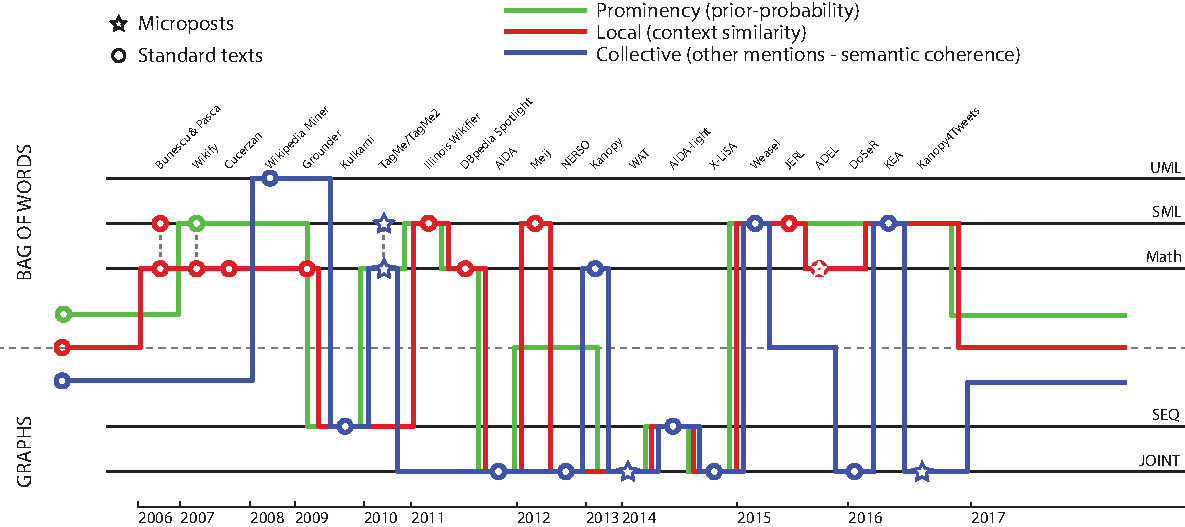
\includegraphics[width=\textwidth]{toolRoadMap}
\end{figure}

\subsection{Prominence Methods.}

To the best of our knowledge, there is not any system that only relies on statistical information or prior probability. A system with this characteristics would be so simple and limited in their effectiveness that there is not much to research in this direction. However, a prominence factor is used in almost every NERD systems, as it favours most frequent entities over more obscure ones with a simple to work with magnitude.

%\subsubsection{Bag-of-words Systems.}

%\subsubsection{Graph-based Systems.}

\subsection{Local Methods.}

\subsubsection{Bag-of-words Systems.}~

\medskip

\cite{mihalcea2007} introduce the term of \emph{Wikification} of a text, that is, convert every relevant mention in a text into a hyperlink to a resource that describes the represented entity. In this case, the resources are Wikipedia articles. This works are based on word sense disambiguation and keyword extraction, so the general approach and many techniques are inherited from these sciences.

This approach is divided in the traditional three steps: pre-processing, keyword extraction (i.e. entity recognition) and word sense disambiguation (i.e. entity linking). ER is performed by querying the surface form dictionary with all the n-grams in the text and then raking it based in up to three different measures. Then, the top \emph{k} candidate mentions are selected as relevant terms, where \textit{k} is determined based on the link frequency in Wikipedia (around 6\% as pointed in the paper). To perform the disambiguation they combine two algorithms in an agreement schema: an annotation is correct when both algorithms say so. First one leverages the similarity between the mention context and the Wikipedia article. The second one uses a machine learning approach based on a Naive Bayes classifier, which uses the context of the mention, its POS tags and some frequent words from the input text as features for the decision making.

\medskip

\cite{cucerzan2007}'s approach leverages contextual information to make the decisions during the disambiguation task. He uses Wikipedia to generate the information about entities, surface forms and categories (these extracted from list pages), although the scope of the system is restricted to named entities only. Recognition of entities is performed with a recognized that uses simple mechanisms like capitalization rules and statistical information to detect the boundaries of the mentions. Disambiguation is accomplished by querying the surface form dictionary to get the candidate entities that could be represented by the gathered mentions. Then, for each mention and candidate entity a vector is generated, which contains contextual and category information about them. Each mention-entity pair is then scored with the scalar product of both vectors, so the pair that maximizes this value (which is not normalized to take in account the prominence of each candidate) is taken as the correct one.

\medskip

\cite{fader2009} give a greater weight to the prominence factor in the ERD process. As pointed before, prominence information by itself is not very reliable, as it has an implicit and unavoidable error margin. However, this error is smaller when an entity is much more probable than the rest, which a frequent fact, so it may be useful to leverage this factor in a general scenario. Moreover, this is how the human mind uses to work.

The authors combine the prominence factor with a contextual similarity measure to perform the disambiguations task. First one is obtained based on the number of wikilinks that point to an article, so the more an article is referenced, the higher will be its prominence value. The contextual comparison is performed through the cosine similarity function (see \autoref{sec:techniques:context}) between the whole input text and the article of the entity. The final score for each mention-candidate entity pair is the product of these values.

\medskip

DBpedia Spotlight (\cite{mendes2011}) is one of the most prominent projects in ERD development. DBpedia Spotlight finds and annotates mentions with DBpedia resources, which is used as the underlying knowledge base. The well-structured DBpedia Ontology let the user to restrict the process to a certain domain, which improves the precision of the system in specific application environments.

DBpedia Spotlight performs both recognition and disambiguation. First, exact string matching is used to look for surface forms in the input text. These surface forms are obtained from the ID labels, redirection pages and disambiguation pages in DBpedia, as well as which resources they link. Then, for each surface form all the candidate entities (and their prior probability for the corresponding mention) are extracted and considered during the disambiguation phase.

Each candidate is represented as a word vector containing all the paragraphs that contain a wikilink to the Wikipedia article that describes the entity. Each word is then weighed with the product of its TF, or term frequency within the resource, and its ICF, or inverse candidate frequency. ICF is a novel measure that indicates the discriminative power of a word: the more resources it is related with, the less discriminative power it has. The context of the mention is represented in a similar manner, so the cosine similarity measure (see \autoref{sec:techniques:context}) can be applied to score the contextual coherence between a mention and each of its candidate entities. Finally, the candidate with the highest score is used to annotate the mention, although we can set a minimum confidence score so only annotations with a higher score than this threshold are performed.

The system was further developed and extended to a multilingual approach in \cite{daiber2013}. This update introduces alternative methods to work with the data in a language-independent manner. During the recognition step, combinations of tokens that form known surface forms are generated and looked for them in the input text, while in the language-dependent implementation some linguistic resources are leveraged, e.g. capitalization or noun phrase detection by POS tagging the input text. Candidate generation remains the same.

Disambiguation is performed using the generative probabilistic model proposed in \cite{han2011generative}. It combines three parameters to calculate a score for each candidate entity: the prior probability of the entity (number of incoming wikilinks), the probability of that the surface form represents that entity (number of wikilinks with the surface form as anchor text that link the entity), and the score of the context of the entity. Then, the candidate with the highest score is selected for each mention.

\medskip

\cite{caliano2016} focus on linking entities in microposts. They rely on a third party NER system to extract all the mentions from the input text, T-NER (see \autoref{sec:erSystems}), but only after pre-processing it accordingly to the nature of this kind of texts. This way, some special characters are removed, like the `\#' or `@' that are common in tweets, and some segments, like hashtags, are transformed into more standardized phrases. 

Then, they obtain, for each mention, the possible resources from DBpedia that could represent the correct annotation. These resources are ranked in function of a \emph{knowledge base score}, so only the top results are retrieved as candidates for a mention. This score is calculated based on three factors:
%
\begin{enumerate*}
\item similarity between mention and the \texttt{rdfs:label} field of the candidate resource (Jaro-Winkler distance, see \autoref{sec:techniques:context}),
\item cosine similarity between the mention context and the description (abstract) of the candidate resource, and
\item popularity measure of the candidate in the knowledge base (Page Rank).
\end{enumerate*} 
%
Finally, the candidate that reaches the highest score is used to annotate the mention.

\begin{comment}

\noindent\rule{\linewidth}{1px}

\tick\nuevaHerramienta{\cite{mihalcea2007} Wikify}
{2007}
{Wikipedia}
{Prominence + Local}
{N-grams}
{Dictionary (exact matching) + Refinement with three measures: TF-IDF, $X^2$ independence test and keyphraseness (prominence)}
{Two methods: Overlapping between contexts; and SML classifier (Naive Bayes) based on prominence.}


\tick\nuevaHerramienta{\cite{cucerzan2007} Cucerzan}
{2007}
{Wikipedia}
{Joint (Local)}
{Capitalization analysis}
{Capitalization rules + Dictionary. Classification in Person, Location, Organization or Miscellaneous. Candidate detection with partial matching.}
{For each possible combination of entity annotations, overlapping between document vector (which aggregates all the contexts and categories of the detected surface forms) and entity vector (which aggregates the Wikipedia contextual information and categories of the selected candidates)}

\tick\nuevaHerramienta{\cite{fader2009} \textsc{grounder}}
{2009}
{Wikipedia}
{Prominence + Local}
{Unknown}
{Unknown (probably dictionary with surface forms taken from Wikipedia)}
{Prominence + Cosine Similarity Function between context of the mention and each candidate entity's context info (combined through Bayes' theorem)}

\tick\nuevaHerramienta{\cite{mendes2011,daiber2013} DBpedia Spotlight}
{2011}
{DBpedia}
{Prominence + Local}
{LingPipe Exact Dictionary-Based Chunker using the surface form catalog}
{Dictionary}
{Cosine Similarity Function between contexts + Prominence + Inverse Candidate Frequency}

\tick\nuevaHerramienta{\cite{caliano2016} UniMiB}
{2016}
{DBpedia}
{Prominence + Local (Microposts)}
{T-NER (Ritter et al.)}
{T-NER (Ritter et al.): CRF}
{Scoring based on popularity of each entity and lexical similarity (both contextual and from the mention)}

\noindent\rule{\linewidth}{1px}

\end{comment}

\subsubsection{Graph-based Systems.}~


\subsubsection{Machine Learning.}~

\cite{bunescu2006} may be considered the first NERD system. This work lays down the foundations for the standard pipeline of mention detection, candidate generation and entity disambiguation, as well as the surface form dictionary linked to the entity catalogue, both generated based on Wikipedia. However, it is restricted to named entities only, that is, those with proper names.

Their approach treat disambiguation as a ranking problem. To solve it, they propose a supervised machine learning approach using support vector machines (see \autoref{sec:techniques:ml}). They use the Wikipedia itself to build many training sets, where the wikilinks in the articles are positive examples, and the candidates that are not linked by them are negative examples. As features for the score calculation, they use cosine similarity, to measure the correlation between each mention's context and the article of each candidate entity, and the Wikipedia taxonomy, to determine the degree of semantic coherence between a mention and the super-categories of each candidate entity. At last, they implement a mechanism to detect and report mentions that do not represent any entity in Wikipedia, which consists on a minimum threshold for the score of the best candidate.

\medskip

\cite{meij2012} was one of the first systems at taking the ERD pipeline to microposts, particularly Twitter. However, this is done at tweet-level, not word-level, so it could be considered as text classification with concepts instead of semantic classes. This system consider as an input every n-gram found in a tweet, so a ranked list of candidate entities is obtained for each one of these candidate mentions in an effort to maximize the recall. To this end they test up to six approaches, being the optimal the CMNS method, proposed by the authors. CMNS measures the frequency with which a n-gram (that is, a surface form) is used as anchor to link a certain concept in Wikipedia, so it is a plain prominence feature. However, it behaves well and provides good results in terms of significance and performance.

For the disambiguation step they implement a supervised machine learning approach with Random Forest as the learning algorithm (see \autoref{sec:techniques:ml}). The training set consists on a number of labeled examples where concepts are annotated with a set of relevant articles. Combining an extensive set of features, the set of candidate concepts that were gathered during the previous phase is re-ranked to select the most relevant ones for the whole tweet.

\cite{yamada2015} take Meij's work as a starting point, and also specialize in microposts. They implement machine learning for the whole ED process, although they use more traditional methods for the ER phase. For this task, they use a dictionary built from Wikipedia data (titles of the articles, redirection and disambiguation pages, and wikilinks' anchor text). This dictionary is queried with all the n-grams from the tokenized tweet through multiple criteria, including exact or approximate match and acronym search.

The resulting mentions and candidate entities are used as input for a supervised model following \cite{meij2012}, although they add  three new features: 
%
\begin{enumerate*}
\item contextual information using word embeddings,
\item temporal popularity knowledge of an entity using the tweet's date and the Wikipedia page view data, and
\item string similarity measure between the mention and the title of the article.
\end{enumerate*}

This system also introduces three novelties: an overlapping resolution mechanism, a NIL mention detection system and the prediction of the mentions' type. The overlapping resolution mechanism is applied after the disambiguation phase, and it analyses if a mention is already contained in a previous one, and only keeps the mention with the greater score and discards the remaining ones. On the other hand, NIL detection is tackled as a classification problem where random forest is used again, but with different features. Finally, mention typing is applied over both NIL and non-NIL mentions using two different machine learning models, which use logitic regression and random forest as learning algorithms, respectively. 

\cite{greenfield2016}'s approach builds over the previous one, \cite{yamada2015}, although this uses DBpedia instead of Wikipedia as the knowledge base. However, the main difference is that they propose an inverse approach for the annotation of entities in tweets: for each entity in the knowledge base, they look for each one of their surface forms in the input tweet. Then, a list of mention candidates is generated for every entity that may appear in the text.

This let us to easily define an specific domain, as well as maintaining their possible surface forms (which could include misspelled forms or frequent variations in this kind of media), because of the top-down approach. Correct spots are determined through machine learning with random forest, same as the works this bases on, but with a more restricted set of features. They experimented with AIDA (\cite{yosef2011}) as their ED engine, but it provided very poor performance when dealing with non-person entities. On the other hand, ER is accomplished through a voting system between multiple recognitions systems.

\medskip

\cite{zheng2012} use Freebase as knowledge base for their proposal. The argument given is that it is richer in entities than Wikipedia. However, it lacks contextual information of them, which is compensated with two features of Freebase: its vast amount of recognized surface forms for its entities, and the rich taxonomy it owns, which make Freebase a more solid information source for both humans and machines.

The authors propose an iterative procedure, where the unambiguous mentions are annotated and later used to disambiguate the remaining mentions. {\color{red}[COMPLETAR]}

\medskip

The proposal in \cite{rao2013} is an EL only system, delegating in third-party tools the recognition of entities in a text. They use Wikipedia as their knowledge base, but try to define a non Wikipedia specific approach in terms of what resources they use from the knowledge base. Their linking pipeline is as follows: first, they gather candidate entities for the input mentions by a string matching method procedure that combines exact matching, overlapping and different similarity measures between each mention and the entries in the surface form dictionary.

After the candidates are identified, they use a supervised machine learning ranker to determine the optimal candidate entity for each mention. They use support vector machines (see \autoref{sec:techniques:ml}) with maximum margin; that is, a candidate entity is selected if it gets the greatest score over every other candidate by a prefixed margin. This should also let us control the confidence of the assignation by tweaking the imposed margin. To make a decision, the system uses a plethora of features about entities, surface forms, Wikipedia features (which would not be present in case of using other knowledge base), etcetera. A novel and interesting magnitude that they take in account is the rank of the Wikipedia article in a Google search as a measure of the prominence or popularity of the entity.

\medskip

\cite{durrett2014}'s proposal uses conditional random fields (see \autoref{sec:techniques:ml}) to tackle the ERD task. They implement entity typing (entity recognition) and coreference detection (that is, detection and clustering of the mentions to a same entity) in conjunction with entity linking in an unique joint pipeline, so every operation can support the remaining to lead to a better result.

For every proposed mention, a list of candidate entities is generated by what is called a \emph{query}: they use not only the whole mention, but all its prefixes to query the surface form dictionary (which is generated based on Wikipedia). Coreference helps ER by ensuring the consistency between the semantic types of similar mentions -- making them to have same POS tags --, but is quite less useful in combination with EL, as the same mention can refer to different entities each time. On the other hand, the combination of ER and EL in a joint task has been pointed by other authors (\cite{luo2015}, \cite{nguyen2016}). There, entity assignments from EL step may provide some information about semantic types thanks to the semantic categories the entities belong to, and vice versa. {\color{red}[REVISAR: ML durillo]}

\medskip

\cite{perera2016} focus an uncommon aspect of the ERD problem: implicit mentions linking. In microposts, the kind of texts this work is oriented to, it is frequent to elide the name of the entity they talk about for the sake of brevity. In these cases, there are no surface forms that could be recognized in the text, so the recall drops to the ground, leading to a poor final result. To overcome from this circumstance, they leverage the contextual information (the tweets that are simultaneously published), temporal salience and factual knowledge.

Contextual information comes from the tweets that are published in a short window of time around the tweet we want to annotate. These tweets may contain not only explicit mentions that may be easily detected and resolved to an entity, but also frequent words or phrases that may be used instead of the implicit mention. Temporal salience is a prominence measure based on the number of views of the Wikipedia article of an entity in the last 30 days. Factual knowledge consists on affirmations and semantic relations with other entities that could be explicit in the tweet. All this information is joined in an Entity Model Network (EMN), whose construction is detailed in the paper.

For the ERD task, the system first generates a reduced model based on the explicit mentions in the tweet. To this end, it queries a surface form dictionary built based on Wikipedia and saves them as ``tweet clues'' to get a graph of candidate entities. This sub-model is used as input for a ranking machine learning model, a SVM, based on pairwise approach; that is, it takes all candidate entity-mention pairs and ranks them in function of which pair is better. To this end, it takes into account the temporal salience and the cosine similarity between the tweet and the entity features (titles of the entities that are connected with the candidate) represented as a vector.

\begin{comment}

\noindent\rule{\linewidth}{1px}

\tick\nuevaHerramienta{\cite{bunescu2006} Bunescu and Pasca}{2006}
{Wikipedia}
{Local}
{Unknown}
{Dictionary (exact matching)}
{Cosine Similarity Function between context of the mention and each candidate entity's context info + SML: SVM Classifier (Naive Bayes) for Wikipedia category correlation}

\nuevaHerramienta{Illinois Wikifier}
{2011}
{Wikipedia}
{Prominence + Local}
{Unknown}
{Manual localization + Dictionary}
{SML Ranking SVM with multiple features: Cosine Similarity Function between contexts, PMI, NGD...}

\tick\nuevaHerramienta{\cite{meij2012} Meij}
{2012}
{Wikipedia}
{Local}
{N-grams}
{Dictionary (exact matching), contextual information or another systems that do NER operations}
{SML (Random Forests Algorithm)}

\nuevaHerramienta{\cite{zheng2012} Zheng et al.}
{2012}
{Freebase}
{Local}
{-}
{-}
{ML. NED only: Semi-supervised, two models: generative and discriminative}

\tick\nuevaHerramienta{\cite{rao2013} Rao et al.}
{2013}
{Wikipedia}
{Prominence + Local}
{-}
{-}
{Supervised ML.}

\tick\nuevaHerramienta{\cite{durrett2014} Durret and Klein}
{2014}
{Wikipedia}
{Local}
{N-grams}
{Grammatical features for the SCRF}
{Structured CRF}

\tick\nuevaHerramienta{\cite{yamada2015} Yamada et al.}
{2015}
{Wikipedia}
{Prominence + Local (Microposts)}
{-}
{Dictionary}
{Random Forest}

\tick\nuevaHerramienta{\cite{greenfield2016} Greenfield et al.}
{2016}
{DBpedia + YAGO}
{Prominence + Local (Microposts)}
{-}
{Dictionary}
{Random Forest}

\tick\nuevaHerramienta{\cite{perera2016} Perera et al.}
{2016}
{DBpedia}
{Prominence + Local (Microposts)}
{-}
{Based on contemporary tweets: they identify the explicit entities and take them as candidates for the implicit entities.}
{Focused on implicit entities (IEL). SVM.}

\noindent\rule{\linewidth}{1px}

\end{comment}

%%%%%%%%%%%%%%%%%%%%%%%%%%%%%%%%%%%%%%%%%%%%%%%%%%%%%%%%%%%%%%%%%%%%%%%%%%%%%%%%%%%%%%%%%%%%
%%%%%%%%%%%%%%%%%%%%%%%%%%%%%%%%%%%%%%%%%%%%%%%%%%%%%%%%%%%%%%%%%%%%%%%%%%%%%%%%%%%%%%%%%%%%
%%%%%%%%%%%%%%%%%%%%%%%%%%%%%%%%%%%%%%%%%%%%%%%%%%%%%%%%%%%%%%%%%%%%%%%%%%%%%%%%%%%%%%%%%%%%

\subsection{Collective Methods.}

Collective methods have been an interesting approach since the early days of NERD, but the first proposals were known for its high computational cost. In consequence, most of the systems that implement collective methods introduce many approximations to alleviate this problem, although the computational exigence of the process has moved from the complexity of the calculations -- as the processors' power has largely increased since 2006 and they can tackle harder problems in less time --, to the scalability of the process.

The introduction of graphs as a tool for solving this problem entailed a great impulse for the collective methods. Graphs not only let us model the needed information in an intuitive manner -- as the entity-relationship model is highly similar to the classic node-edge graph, directed or not --, but they also provides a set of algorithms and procedures that are common in graphical processing.

\subsubsection{Bag-of-words Systems.}~

\textsc{TagMe} \cite{ferragina2010} is one of the most successful systems that carries out the ERD-in-microposts problem. Its main goal is to provide with a system that is capable of annotate short texts --in this case, tweets-- with Wikipedia articles on-the-fly, that is, in almost real time. As we pointed before, the generation speed of microposts is very high, so a very agile and light processing is required to annotate them as they are generated.

Both the surface forms and entities are gathered from Wikipedia. For each surface form, they register the proportion of times it is used as anchor text in a wikilink (\emph{link probability}); and the probability of it linking each one of its possible candidate entities (commonness or prior probability). They do not indicate any procedures for the recognition, so we assume that mentions should be tagged in the input text.  Candidate entities are generated by querying the surface form dictionary and retrieving all the possible senses for each one of them. Then, this candidate senses are scored and ranked to determine the optimal one. 

The scores are generated through a voting scheme: for each candidate sense, all the candidates of the remainder mentions are analysed to measure the relatedness between them (in case a mention have more than one candidate, they calculate the average relatedness score for all its candidates, which are pondered with their prior probability) and said candidate sense. The proposed relatedness measure is Milne and Witten's function (see \autoref{sec:techniques:semantic}).
\begin{comment}
, the formula being:
%
\begin{equation}
\mathrm{vote}_b(p_a) = \frac{\sum_{p_b \in P_g(b)}{} rel(p_b,p_a)\cdot P_r(p_b|b)}{|P_g(b)|}
\end{equation}
\end{comment}

To this end, they propose two algorithms:
%
\begin{enumerate}
	\item Disambiguation by classifier: A classifier that combines commonness and the relatedness score of each candidate to generate a ``probability of correct disambiguation'', and assigns that with the highest score.
	\item Disambiguation by threshold: This algorithm selects the top \textit{k} candidates in base to their relatedness score and recalculates its score after discarding the remainder senses. Then the one with the highest score is used to annotate the mention.
\end{enumerate}

Finally, a pruning phase is performed over the result set to discard irrelevant mentions. For each mention, a value is generated using two parameters: the link probability of the mention, and the coherence between the annotated entity and the entities used for the remainder of the mentions. The calculation of this value can be carried out with an arithmetical combination of both factors, or through a machine learning classifier (SVM and C4.5 are mentioned as possibilities). This way, all the mentions that are not coherent with the rest of the text are deleted from the final result.

\textsc{TagMe} was updated and received its version 2.0 in \cite{ferragina2012}. There they describe a pre-processing and recognition algorithm, which the past version lacked, that consists on extracting a set of n-grams from the text and removing those that do not bring any result when querying the surface form dictionary. Then, overlapping between mentions is solved by keeping the longer ones, unless the shorter ones has a much bigger link probability. 

The disambiguation phase remains unchanged, including both disambiguation algorithms, but they add two thresholds for the values of link probability and commonness of the candidate mentions and candidate entities, respectively, to tune the process in order to improve the accuracy or the efficiency with a minimal trade off with the recall.

\medskip

\cite{scaiella2014} propose DataTXT, presented as the evolution of \textsc{TagMe}. DataTXT keeps the general pipeline and algorithms of \textsc{TagMe}, but adds some new features and improvements. For instance, during the disambiguation step a new parameter is introduced to weigh the influence of context and commonness (prior probability). The rest of changes are different adaptations to the requisites of the Microposts 2014 challenge, to which DataTXT was one of its contestants.

\medskip

\cite{hulpus2013} describe Kanopy, an ERD system that leverages the DBpedia's semantic network to generate additional wealth from natural language texts beyond the mere entity linking. Kanopy generates a graph that semantically describes the whole input text, and provides with a semantic contextualization of the recognized concepts, as well as a list of the most relevant topics in the text. First, it extracts the relevant phrases from the text, i.e. noun phrases through Stanford CoreNLP. Then, it cluster them depending on the topics behind these phrases using diverse techniques.

The ERD task is performed using WSD and Eigenvalues (see \autoref{sec:techniques:semantic}), described by the authors in \cite{hulpus2012}. From the set of DBpedia resources used to annotate the mentions, Kanopy build a graph by expanding two levels an initial graph that contains them all. This graph is used to generate the most relevant concepts by performing a ranking algorithm to measure the semantic centrality of each node that corresponds with an annotated resource.

\medskip

\cite{liu2013} tackle the entity linking in short texts by leveraging three types of coherence -- mention-entity, entity-entity and mention-mention -- to provide result that maximizes the coherence between each one of the annotations, following the hypothesis that all entities in a text should be related to some extent. This systems only performs ED, so the input text should already have all the mentions tagged manually or by using another ER system.

Candidate entity generation is performed by looking at the surface form dictionary. For each candidate entity, a score is generated using three parameters:
%
\begin{enumerate}
\item Mention-entity similarity: Many features are used to model this score, which include prior probability over the set of Wikipedia's wikilinks, the proportion of words that are common to both the tweet and the Wikipedia article, and some binary factors that indicates the edit distance similarity, and whether the mention contains the title of the entity, or the title of the entity contains the mention.
\item Entity-entity similarity: In order to obtain this value, authors use the Milne and Witten formula (see \autoref{sec:techniques:semantic}).
\item Mention-mention similarity: Some string comparisons are performed over each pair of mentions, e.g. cosine similarity or the edit distance between them; and two contextual features that point whether both mentions belongs to tweets from the same account, and whether both mentions contain a common hashtag.
\end{enumerate}
%
These values are pondered with some additional parameters that do not depend on the input text, but are prefixed or obtained from a training set instead. The set of entities that maximize the sum of all its values is selected as the correct assignations for the input set of mentions.

\medskip

\cite{sodergren2017}'s proposal belongs to the multilingual approach for ERD. This system leverages Wikipedia to obtain entities and surface forms, but also uses Wikidata as the central entity repository in order to get access to the structured data it contains, like dates, and its multilingual information. Additionally, some features are gathered to use them during the annotation process: prior probability of each entity with respect to a mention, an approximation of the ambiguity of each mention, if there are proper names or stopwords in a mention, etcetera.

Mentions are spotted by looking for any known surface forms from the dictionary in the input text. The results are pruned by applying some simple manually-written rules to remove irrelevant mentions in order to improve the precision, but trying to without harming the recall. Some examples are capitalization analysis or a threshold for the link probability of a mention (the frequency with which it acts as a wikilink over all its appearances in Wikipedia).

For the disambiguation step they apply the Page Rank algorithm up to three times over an undirected graph where each mention-entity pair is included as a node, and the nodes are linked when %
\begin{enumerate*}
\item the article of one entity has a wikilink to the article of another entity in the graph, or
\item two links to both entities are found in a same paragraph in Wikipedia.
\end{enumerate*}
%
After this step, all the nodes should have a score. Then, a weighted category graph -- generated by relating each article in Wikipedia with its main categories along all its versions in other languages -- is used to determine the coherence between each candidate article and the set of categories of the core entities in the text, i.e. those that do not present ambiguity.The highest scored entities for each mention are used to perform the annotation. 

{\color{red} [REVISAR: Confuso. Ver \cite{eckhardt2014}, en el que se basan estos señores.]}

\begin{comment}

\noindent\rule{\linewidth}{1px}

\tick\nuevaHerramienta{\cite{ferragina2010,ferragina2012} TagMe/TagMe2}
{2010}
{Wikipedia}
{Prominence + Collective (Microposts)}
{N-grams}
{Dictionary}
{Prominence + Collective agreement between the candidate entities (M\&W). This values are combined through one out of two methods: Disambiguation by classifier (ML), or Disambiguation by Threshold.}

\tick\nuevaHerramienta{\cite{hulpus2013} Kanopy}
{2013}
{DBpedia}
{Collective}
{Stanford CoreNLP}
{Stanford CoreNLP NER + Noun phrase clustering phase}
{Word Sense Disambiguation usin eigenvalues}

\tick\nuevaHerramienta{\cite{liu2013} Liu et al.}
{2013}
{Wikipedia}
{Prominence + Local + Collective (Microposts)}
{-}
{-}
{Ranking with prior, context similarity, co-ocurrence of mentions and M\&W among others.}

\tick\nuevaHerramienta{\cite{scaiella2014} DataTXT (evolution of TagMe)}
{2014}
{Wikipedia}
{Collective (Microposts)}
{-}
{Dictionary}
{Scoring}

\tick\nuevaHerramienta{\cite{sodergren2017} HERD}
{2017}
{Wikipedia + Wikidata}
{Local + Collective (Multilingual)}
{-}
{Dictionary: Solr Text Tagger + Lucene}
{Scoring: PageRank + Category coherence}

\noindent\rule{\linewidth}{1px}

\end{comment}

\subsubsection{Graph-based Systems.}~

\cite{kulkarni2009} introduce the graphical approach into the ERD task. Apart from providing with a somewhat intuitive representation of mentions and entities, it brings us the possibility of measuring the semantic coherence between the candidate entities by jointly considering them in the disambiguation problem.

This system builds over Wikipedia as the source for the entity catalogue and the list of surface forms for each entity. Mentions are extracted through partial matching between segments in the input text and a surface form from the dictionary. Four pieces of information are gathered for each entity: both the introduction paragraph and the full Wikipedia article, the set of all anchor texts used to link this article, and a context for each one of these anchors. Authors use this data to measure the contextual similarity between a mention and each of its candidate senses. Both contexts are compared through different measures to improve the confidence. A prior probability factor is also considered based on the frequency with which a surface form is used in Wikipedia to link a specific article.

A novel factor in this work is the relatedness degree between entities, whose calculation relies on Milne and Witten's WLM to determine the pair-wise semantic coherence. Then, the challenge is to find the assignment that maximizes the combination of contextual and semantic coherence. Here lies the downside of the graphical approach: the computational cost may be very high. To this end, authors propose two approximations (a LP rounding approach and a hill-climbing algorithm), which are compared with a context-only approach as the baseline. Although both algorithms brings better results than the baseline, there is not a clear winner: first one provides with better results, but the latter is more lightweight. This is an habitual trade-off in this kind of environments.

\medskip

\cite{yosef2011} present AIDA, one of the most prominent proposals in ERD development. AIDA is characterized by its powerful, yet computationally heavy, recognition and disambiguation pipeline, which brings accurate results by making use of a complex graphical model. Its graphical approach allows to use both statistical, contextual and semantic coherence data to find the densest subgraph that contains the optimal combination of annotations for the observed mentions.

AIDA's pipeline is further explained in \cite{hoffart2011}. First, mentions are discovered by using Stanford NER Tagger, which yields a high precision, high recall input for the candidate generation step. Candidates are obtained from YAGO, a knowledge base that is developed by the authors of AIDA, by looking for the observed mentions among the surface forms that are stored in YAGO. Then, each candidate is scored with a function that combines prior probability of each candidate given the found surface form, the similarity between the mention's context and the stored contextual information of the candidate entity, and the semantic coherence between all the candidates. These parameters are weighed accordingly to the values obtained from a SVM classifier.

To tackle this optimization problem, authors choose to implement a undirected graph-based method. Both mentions and candidate entities are included as nodes. Then, two types of edges are created: mention-entity edges, and entity-entity edges. Then, mention-entity edges are weighed with the similarity between the mention and the entity based on their context: the input text for the mention, a set of key phrases for the entity (e.g. titles and anchor texts from Wikipedia). Entity-entity edges are weighed using Milne and Witten's WLM.

Once the graph is constructed, the optimal combination of annotations that maximizes the objective function must be found. However, this problem is NP-hard and must be tackled by using an approximation. First, a distance to its mention node is calculated for every entity node, so only the closest $n$ nodes are kept and the remainder are removed from the graph. Then, authors apply a progressive pruning of the least significant candidate for the set of mentions, unless it is the last candidate for a mention (\emph{taboo node}). After each deletion, values from all the nodes are updated. When each mention has only one candidate entity, that graph contains the optimal mention-entity assignation for the input set of mentions. An alternative local-search approach is also proposed, where candidate entities for each mentions are randomly selected by using its weights as a ``jumping probability'', and repeating this process a fixed number of times, although this method ignores coherence between entities.

\medskip

\cite{han2011} go beyond \cite{kulkarni2009} and propose a global interdependence model in opposition to their pair-wise coherence approach. To this end, they construct a graph, the Referent Graph, that aims to capture both the similarity between a mention and a candidate entity and the coherence in the set of all candidate entities for every mention in an input text. Mention nodes are connected with their candidate entity nodes, and then each pair of entity nodes are linked with a undirected, weighed edge if there exists a semantic relation between them.

Mention-entity correspondence degree is measured by analysing the co-occurrence of words in their respective contexts, represented by two vectors where each word is weighted with its TFIDF score. The context information for each entity consists exclusively on its Wikipedia article. On the other hand, semantic relation between entities is scored with Milne and Witten's WLM.

The disambiguation model can be presented as a random walk with restart on graphs approach. First, each candidate is scored based on its \emph{prior importance}, i.e. its TFIDF score, as a form of relative pre-ranking of the candidates. These values will be used as the \emph{initial evidence} of the correct annotation for the input mention set. A matrix is constructed with the factors that weigh each pair of candidate entities in the referent graph, where each value can be seen as the hop-probability between two nodes. If a node has not outgoing relations, i.e. is not connected to any other candidate entity, a \emph{restart} is performed to avoid to interrupt the evidence propagation and its disappearing at that node. This restart consists on transferring a part of the propagating evidence to the initial evidence after every step. This way, initial evidence is propagated though the set of candidates, so a accumulated value is obtained for each candidate entity. Then, the candidate with the highest score is used to annotate each one of the input mentions.

\medskip

\cite{hachey2011} bring a WSD approach to entity linking. They propose a theoretical graph with all the articles and categories from Wikipedia by leveraging its wikilinks' structure. First, candidates are generated by querying the index of entities, that is, looking for Wikipedia titles that match each mention from the input text. Then, a subgraph that contains all the candidate entities, as well as all the intermediate nodes that form paths between the said nodes, is extracted from the global graph. To keep the graph size under control, they impose a fixed maximum path length, which is set to 2 for entity nodes, and 3 for category nodes.

Then, the goal is to score each node in the graph to determine the optimal correspondence. They propose two graph measures to score each node: Degree centrality and Page Rank, which are combined with cosine similarity as contextual comparison measure. Degree centrality is the proportion of incoming edges of each node over the total of nodes minus one. Page Rank has its usual formulation. ({\color{red} Verificar.}) On the other hand, cosine similarity is calculated between the paragraph where the mention is, and the whole Wikipedia article that describes a candidate entity. The entity with the highest score is selected as the correct one for each mention.

\medskip

\cite{hakimov2012}'s NERSO, which stands for Named Entity Recognition Using Semantic Open Data, performs recognition and linking using DBpedia and a graphical approach. They use a centrality measurement algorithm to identify the correct entity for each one of the ambiguous mentions in an input text. First, they perform a spotting step, where a sliding window is applied on the input text in search of segments --sets of consecutive words-- that matches the titles of the DBpedia resources that form its surface form dictionary. This sliding window has a fixed initial length that is reduced if a segment does not correspond to any known surface form.

The graph is built using the {\smaller \texttt{dbont:wikiPageWikiLink}} from DBpedia, which are ultimately obtained from the wikilink set from Wikipedia. This originates a directed graph where all the candidate entities are represented as nodes, and the edges are created based on its links to other candidate entities in DBpedia. On this graph, they apply a centrality scored method where the score for each node is the number of reachable nodes from it --that is, the nodes to which there exists a path--, divided by the sum of the lengths of the shortest path to each one of them. The method that is used to determine these path's lengths is the Djikstra's algorithm.

This centrality score is combined with the number of incoming links, outgoing links and a factor that indicates the type of node to generate the final score. Then, the highest scoring candidate entity is assigned to each spotted mention.

\medskip

In \cite{hakimov2016}'s NERFGUN, authors take some ideas from previous works and expand them by looking at other proposals in the state of the art. They propose an undirected, probabilistic graphical approach which makes use of prominence, contextual similarity and semantic coherence between candidates during its pipeline. NERFGUN is a pure NED tool, thus it requires the mentions to be labeled before it starts the process. Candidates are retrieved by querying a dictionary, which is built using both DBpedia and Wikipedia, the first to gather named entities and some surface forms, and the latter to enrich the surface form dictionary using wikilinks' anchor texts.

NERFGUN uses factor graphs \cite{kschischang2001factorgraphs} to discover the correct disambiguation for the ambiguous input mentions. The factor graph includes both mentions and textual clues (tokens from the text for context comparison purposes) as \emph{observed variables}, and the set of entities that are referred to by these mentions as \emph{hidden variables}. The goal is to discover the optimal values for these hidden variables. To this end, they propose an optimization approach, where a random combination of candidate entities is taken as an initial step. Then, this assignation is iteratively transformed as follows: in each step, a set of combinations are generated by changing the current combination in only one mention annotation; from this set, the best combination is selected and passed to the next iteration. If no new combination is better than the current combination, it is kept. This procedure is repeated for a fixed number of iterations.

Generated combinations are scored by using a probability distribution function that comprises many factors:  entity frequency for a given mention, edit similarity --the Levenshtein distance between a mention and an entity--,  document similarity -- cosine similarity between the text and the initial paragraph of the Wikipedia article for an entity--, and two variants of Page Rank that aim to measure the popularity of the entity in Wikipedia and the semantic coherence between the entities used in a combination. After the iterative process, the resulting combination should be a correct assignation for the input mentions.

\medskip

\cite{nguyen2014} adapt the works in \cite{yosef2011} to a light-weightier pipeline to overcome its scalability issues, given the complexity of its computation process. They develop a thematic domain approach, which evaluates semantic coherence between entities by analysing its categories in a predefined ontology. Contextual information is introduced in the process by leveraging the fact of some mentions being unambiguous, so they constitute a solid ground to help to disambiguate the remaining mentions in a text.

AIDA-light starts with a text where the mentions has already been recognized and labelled. Then, a set of candidates is generated for each mention by querying a surface form dictionary. The exact matching method between mentions and surface forms is not indicated, but we can assume that is a partial or approximate matching. For each mention, two word sets are constructed for both the surrounding mentions and tokens for each mention. Then, unambiguous (``easy'') mentions are used to determine the domains which the input text belongs to, so these domains are added to the mention context of the remaining mentions. On the other hand, entities need to have a context set of words, which is filled with key tokens from their YAGO resources.

Disambiguation algorithm requires the combination of two dimensions:
%
\begin{itemize}
\item Mention-entity features: They include prior probability, mention-entity name similarity (based on the Jaccard coefficient between the mention and the entity name), mention-entity context similarity (using word overlapping between the token context and the key tokens of the entity), surrounding mention coherence (measured by the co-ocurrence in Wikipedia of the unambiguous entity and each one of the candidates), and the coherence between entities (by measuring the overlapping between their key tokens).
\item Domain-oriented features: They relate to the defined domain hierarchy, like the distance between the categories which two entities belong to.
\end{itemize}
%
Both sets of features join in an objective function, which lets us to score in a joint manner every candidate entity for the considered mention set. Disambiguation happens in two stages: first, only ``easy mentions'' are used as input on their own, excluding the remaining mentions (those with $\geq4$ candidates), and a graph is constructed using the top k entities, i.e. entities which bring the highest similarity value with the mention by using only its local features. Then, entities with the lowest entity and domain coherence are iteratively removed, recomputing the scores for the entities in each step. This is repeated until each mention has only one candidate entity. In the second stage, domains in the text are determined using the already disambiguated mentions. Then, the previous procedure is applied to the entities that remain ambiguous.

\medskip

\cite{usbeck2014agnostic,usbeck2014graph}'s approach, AGDISTIS, is a graph-based, knowledge base agnostic NED system. This fact requires a previous index creation step, where entities and their respective surface forms are gathered from the chosen knowledge base. Starting with a text where the mentions are already labelled, AGDISTIS generates candidates for each mention by using exact matching in the surface form index. Then, a two-step process is performed on the mentions: first, string normalization reduces each mention to its root, removing variations like plurals, genitives and time information; second, term expansion allows establishing relations between the mentions in text that point to the same entity. Reasoning behind this is that it is common that only the first reference to an entity is a complete surface form (e.g. name and last name: Bruce Springsteen), being the following mentions a substring of the first one (e.g. last name only: Springsteen). This is a simple implementation of \emph{coreference resolution} in a text. This way, the number of mentions that must be disambiguated can be drastically reduced. Finally, normalized mention and entity name are compared by using trigram similarity to measure their textual fitting to avoid noisy results by removing little relevant candidates.

To disambiguate between candidates, AGDISTIS builds a directed graph where candidates are included as nodes and edges are relations between pairs of entities, somehow defined in the underlying knowledge base (e.g. there exists a RDF triple that links them). Then, this graph is expanded in an iterative manner by adding the nodes from the KB that are related with the nodes already in the disambiguation graph. Lastly, HITS algorithm (see \autoref{sec:techniques:semantic}) is performed over this graph to rank the candidate nodes for each mention and to select the most authoritative one as the correct annotation.

\medskip

\cite{piccinno2014}'s WAT is a rework of \textsc{TagMe} in order to make its architecture modular and more efficient, and all its algorithms are revised. It keeps Wikipedia as its knowledge base, and all the structures that \textsc{TagMe} used to perform the ERD task. First, WAT analyses the input text looking for words or phrases that match one entry in the surface form dictionary. They also propose an optional binary SVM classifier that helps to determine if a mention is relevant or not.

Apart from the one that is implemented in \textsc{TagMe}, WAT propose a novel group of graphical algorithms, following the success of AIDA with these techniques. In it, both mentions and entities are represented as nodes, and between them there exist two types of edges: mention-entity, to describe the condition of candidate of the latter, and entity-entity, to indicate the fact that two entities are semantically related. The edges mention-entity can be weighted one out of three measures:
%
\begin{enumerate*}
	\item identity (weight always equal to 1),
	\item commonness (prior probability), or
	\item context similarity between the mention's context and the Wikipedia article.
\end{enumerate*} 
%
On the other hand, the edges entity-entity are weighted with the Milne and Witten's relatedness measure (see \autoref{sec:techniques:semantic}). They propose many algorithms to generate a score for each candidate entity, like Page Rank. For the pruning step, they train a SVM binary classifier to decide whether a mention is relevant or not, in addition to the pruner from \textsc{TagMe}.

\medskip

\cite{zhang2014} try to overcome the language problem of NERD by proposing a cross-lingual approach. Working in a multi-language environment greatly increases the amount of surface forms that need to be considered, so it could be difficult to determine which segments of a text are effectively mentions, and with which entity they should be annotated. A mono-lingual approach could also lead to miss many mentions that are expressed in a distinct language than the text's dominant one. Authors propose a model where information is represented in multiple languages based on multilingual Wikipedia and DBpedia \cite{zhang2014xlid}. For each entity in DBpedia, which is the grounding for their knowledge base, they gather all surface forms for that entity over the multiple versions of Wikipedia, as well as frequency statistics. Information in every language is then aligned to let an easy transposition from one language to the reference language.

Mentions are discovered through the analysis of the n-grams in an input text. In case of ambiguity a disambiguation algorithm is performed, which utilizes two kinds of features. These values will be introduced in a directed graph where mentions and candidate entities are included as nodes. Edges are introduced from mentions to entities, and between every pair of entities that are connected. First, mention-entity semantic similarity combine two different features: link probability as the prominence factor, and the value of cosine similarity between the mention's context and the entity's description vector in the reference language. The resulting value is used to weigh mention-entity edges. Second, entity-entity coherence is obtained by calculating the semantic relatedness between each pair of entities. To this end, authors use Normalized Google Distance over the wikilink structure from Wikipedia, an adaptation of Milne and Witten's approach.

On this graph, they perform a personalized Page Rank algorithm, which assigns a probability score to each entity node. Then, for each mention they assign the most probable entity to it.

\medskip

\cite{plu2015hybrid,plu2015revealing} propose a hybrid approach in three phases: recognition, linking and pruning. For the ER task, they rely on the Stanford NLP tools, more specifically the POS Tagger and the NER system in combination with two gazetteers for job names and nationalities (which help in the disambiguation step). The training details for these systems are detailed in the citation.

This system leverages both Wikipedia and DBpedia to generate an index of entities with a set of features, which will be used during the disambiguation and pruning steps. First, it builds a graph with all candidate entities, and the context of all of them -- that is, the articles pointed by the outgoing wikilinks. Edges are weighted based on the absolute frequency of each wikilink to another candidate entity as a context coherence measure.

Then, a score is generated for each candidate entity by a function that combines a linear combination string similarities of the mention with the article title, the redirect pages and the disambiguation pages, with a Page Rank score. Finally, they propose a supervised learning approach that lets the system be adaptable to different domains through its training data. To this end, they use a classifier that discards all the annotated mentions that do not match the domain defined in the labeled data used to train the system.

This system is later named ADEL and further developed in \cite{plu2016}.

\medskip

\cite{zwicklbauer2016doser,zwicklbauer2016robust} propose DoSeR, a knowledge-base-agnostic system for performing EL in a general domain. This is accomplished by implementing semantic embeddings into the disambiguation process to standardize the contents from every used knowledge base. To this end, DoSeR requires an initial step where the selected knowledge bases are processed into an unified entity index. Both RDF (DBpedia, YAGO) and document-oriented (Wikipedia) knowledge bases are compatible.

These knowledge bases are divided in two groups: core KBs, which will be used to gather the entities that will integrate the entity catalogue, as well as many other data, and optional KBs, which will provide complementary information as additional surface forms. For each entity, an entry with three fields is created: label, or primary name for the entity; prior probability, which is its relative frequency along the knowledge bases; and the semantic embedding, or vectorial form of the entity. To create these vectorial representations, they use Word2Vec (see \autoref{sec:techniques:other}).

Disambiguation algorithm is as follows. First, mentions must be labelled in the input text in order to be processed by DoSeR. All the dictionary entries that match a mention provide entities to the candidate list, although only the most relevant ones are included to improve the efficiency of the process. To this end, all candidates that does not exceed a given threshold on a trigram similarity calculation between their labels and the mention are removed.

Candidates are introduced in the entity candidate graph: a complete, directed K-partite graph, where each of its K subsets corresponds to one input mention. Entity-entity edges are created only between nodes that belong to different subsets. These edges are weighed with the cosine similarity between their respective embeddings. These values are then used as transition probabilities in the random walk algorithm that is performed to score the candidate entities, and provide us with the collective dimension of EL. After that, the entity in the highest-scored node in each subset is selected as the correct annotation for the corresponding mention.

\medskip

\cite{torres2016} adapt Kanopy to specialize it to microposts, more specifically tweets from Twitter. However, this system, Kanopy4Tweets, is also able to process standard text with relative success, as they implement two different pipelines, one for each kind of text. Kanopy4Tweets perform a full NERD pipeline by integrating TwitIE\cite{bontcheva2013} (see \autoref{sec:erSystems}), a modified version of GATE's ANNIE to let it process tweets, or directly ANNIE to operate on standard texts. This step is what lets Kanopy4Tweets be able to process tweets, as the rest of the pipeline is not particularly specialized in this kind of texts.

DBpedia is used as knowledge base to get both the entities list and their surface forms. Candidates for the mentions are generated in an iterative way, imposing an exact mention-entity name matching in the first iteration and relaxing this requisite in the following until at least one candidate is located. If there are no candidates, NIL resource is used to annotate that mention. If the list of candidates is too large, they select only the most relevant results for the disambiguation step. This task is performed by Kanopy, which provides a graph where the mentions are linked to their best candidate entity.

\begin{comment}

\noindent\rule{\linewidth}{1px}

\tick\nuevaHerramienta{\cite{kulkarni2009} Kulkarni}
{2009}
{Wikipedia}
{Joint (Prominence + Local + Collective)}
{Unknown}
{Manual localization + Dictionary}
{Optimization problem in a probabilistic graph model, weighted by two features: mention-entity, and entity-entity}

\nuevaHerramienta{\cite{yosef2011} AIDA}
{2011}
{YAGO}
{Prominence + Local + Collective}
{Stanford CoreNLP}
{Stanford NER}
{Densest sub-graph that maximizes the coherence between candidate entities (iterative pruning of the least probable candidate entity)}

\tick\nuevaHerramienta{\cite{han2011} Han, Sun, Zhao}
{2011}
{Wikipedia}
{Local + Collective (Joint)}
{-}
{-}
{EL only: Interdependence graph E-M and E-E}

\tick\nuevaHerramienta{\cite{hachey2011} Hachey et al.}
{2011}
{Wikipedia}
{Collective}
{-}
{-}
{EL only: Parallelism between NEL and WSD. Unsupervised methods based on graphs (wikilinks and categories).}

\tick\nuevaHerramienta{\cite{hakimov2012} NERSO}
{2012}
{DBpedia}
{Local + Collective}
{N-grams (sliding window)}
{Dictionary (exact matching)}
{Construction of a directed graph with entities and relationships between them + Centrality score (taking in account the number of adjacent nodes and distances to any other reachable node in the graph)}

\tick\nuevaHerramienta{\cite{nguyen2014} AIDA-light}
{2014}
{YAGO}
{Prominence + Local + Collective}
{Tokenization + Porter lemmatization algorithm}
{Stanford NER}
{Graph weighted with the next combination: Prominence + mention-entity similarity (Jaccard coeficient over trigrams + overlapping between their contexts) + entity-entity (overlapping between their contexts + domain and category coherence)}

\tick\nuevaHerramienta{\cite{piccinno2014} WAT}
{2014}
{Wikipedia}
{Prominence + Local (only graph-based algorithm) + Collective  (Microposts)}
{Unknown}
{}
{Voting algorithms, or a graph-based algorithm (which uses prominence, context similarity through BM25 and entity coherence through M\&W)}

\tick\nuevaHerramienta{\cite{zhang2014} X-LiSA}
{2014}
{Wikipedia + DBpedia}
{Prominence + Local + Collective}
{N-grams}
{Dictionary}
{Weighted graph}

\tick\nuevaHerramienta{\cite{plu2015hybrid,plu2015revealing,plu2016} ADEL}
{2015}
{DBpedia + Wikipedia}
{Collective (Microposts + Standard)}
{-}
{Linguistic: Stanford NER and POS Tagger to get proper nouns, then dictionaries}
{Densest weighted graph. Final step is a pruning phase.}

\tick\nuevaHerramienta{\cite{zwicklbauer2016doser,zwicklbauer2016robust} DoSeR}
{2016}
{Agnostic}
{Collective (Joint)}
{Unknown}
{Manual + Dictionary}
{Weighted graph + Random walks}

\tick\nuevaHerramienta{\cite{torres2016} Kanopy4Tweets}
{2016}
{DBpedia}
{Collective (Joint) (Microposts)}
{Unknown}
{TwitIE}
{Weighted graph based on coherence between candidate entities}

\tick\nuevaHerramienta{\cite{hakimov2016} NERFGUN}
{2016}
{DBpedia + Wikipedia}
{Collective}
{-}
{-}
{NED only. Undirected probabilistic graphs}

\noindent\rule{\linewidth}{1px}

\end{comment}

\subsubsection{Machine Learning.}~

\cite{milne2008}'s main objective is to automatically create the cross-references between two Wikipedia articles, i.e. to apply the ERD pipeline on Wikipedia articles. They propose an inverse approach, where disambiguation is performed before the recognition, so only relevant entities would be seen as mentions and annotated in the input text. That is, they do not want to detect all the possible mentions, but only the relevant ones.

They train a machine learning classifier with all the wikilinks in Wikipedia (which are a huge set of manually labelled training data). This system takes as input all the n-grams in the document, and processes them all without distinction. Three features are obtained during the learning process:
%
\begin{enumerate}
	\item Commonness: The frequency with which an article is linked with a certain anchor text (surface form). This value is obtained from the links in Wikipedia, and acts as a prominence measure or prior probability.
	\item Relatedness: The degree of similarity between an article and each one of the articles that are linked in it (which act as unambiguous links). This value is measured through the Milne and Witten relatedness function (see \autoref{sec:techniques:semantic}) \cite{witten2008}.
	\item Context quality: This value balances commonness and relatedness, in a way that favours the relatedness for the uncommon candidates, and the commonness when the relatedness between articles is low.
\end{enumerate}
%
After this step, no articles are selected yet. For each candidate article an annotation probability is generated, which used in the next step as a feature for a new ML classifier in combination with other four features:
%
\begin{enumerate*}
	\item Link probability: Average and maximum values of every article that may be linked by a certain anchor text.
	\item Relatedness: Same as used during disambiguation.
	\item Disambiguation confidence: The maximum and average probabilities of the candidate articles of an n-gram.
	\item Generality: Depth in Wikipedia's categories tree.
	\item Location and spread: Describe the frequency and dispersion of the links to a certain article in the input text.
\end{enumerate*}
%
All the n-grams with a higher value than a pre-fixed threshold are annotated with the most probable article, according with the disambiguation model's results.

\medskip

\cite{chang2014}'s E2E is an ERD system specialized in microposts using Wikipedia and Freebase as knowledge bases. Pre-processing and candidate generation are pretty standard -- input texts are tokenized, and the result is analysed in search of surface forms from a dictionary (the criterion is based on approximate matching to improve recall). Each one of this surface forms has a set of associated candidate entities, which will be evaluated during the disambiguation phase. During tokenization, text is normalized by removin special characters like `@' or `\#'.

All the tokens are considered during the recognition and disambiguation, as well as all the candidates for each one of them. Both tasks are performed jointly: for each token, an annotation will be generated (with an actual resource or a NIL resource, if it has no candidates), but only those annotations that are considered valuable are included in the final result. The scores are generated using a supervised machine learning method (SVM or MART gradient boosting algorithm, see \autoref{sec:techniques:ml} for further information). Feature sets are the following:
%
\begin{enumerate*}
	\item textual features that characterizes the surrounding context of the mention,
	\item entity graph features, which capture the cohesiveness between entities and possible annotations, and
	\item statistical features, which include the entity popularity or word frequency.
\end{enumerate*}

Then, top scorer candidates are used to annotate the mentions. It is not pointed in the paper, but we can assume a minimum threshold for the candidates, so the mentions that have not any candidates with a higher score are annotated with NIL, i.e. discarded from the final result.

\medskip

\cite{luo2015}

{\color{red} Este no lo incluí ni en el TFG, no entendía bien el proceso. Me perdía entre la parafernalia matemática.}

\medskip

\cite{waitelonis2016} present KEA, a machine learning system to perform EL on microposts. KEA uses DBpedia as knowledge base, but also leverages the wikilink structure from Wikipedia through a graphical approach. For the pre-processing and recognition steps they rely on modules from the state-of-the-art Stanford CoreNLP (Log-linear tagger and NER). The text is tokenized and a set of n-grams (segments) are generated as candidate mentions. Candidate entities for each of these n-grams are obtained by exact matching from a surface form dictionary, build from DBpedia entities' labels. Overlapping between mentions is resolved by selecting the longer segments.

Then, a score is generated for each candidate entity using two groups of features:
%
\begin{enumerate*}
\item local features compare the segment and the candidate entity: string similarity, prominence of the entity, semantic coherence between types, etcetera; and
\item context features, which relate the candidate entity with the candidates for other mentions in a given context; wikilinks or links in DBpedia between two entities are examples of these features.
\end{enumerate*}
%
Then, the scores are normalized and the candidates with the highest values are used to annotate the mentions.

\medskip

\cite{nguyen2016}'s J-NERD performs ER and ED tasks jointly, so they can help each other in the decision making during the process. This way, they aim to avoid many problems that the traditional two-staged pipeline implies, like the error propagation from recognition to disambiguation. In this approach, sentences are individually processed using linear-chain and tree shaped probabilistic graphical models, and then integrated in a global model to generate the final result.

Two approaches a proposed to implement the local processing step. Linear model implements a CRF model that takes a sentence as a vector of tokens, and creates a theoretical solution variable that is the correct entity assignation for each one of them. Each solution variable depends on the previous and next variables with a weighed relation (semantic coherence). Tree-shaped model, however, establishes relations between solution variables whose tokens are related by its type, which is assigned by the used Stanford parser.

Both are later integrated in a global model that considers all the sentences in the input text and let the system to discover relations between entities based on the coincidence of their respective tokens (mentions). With this global model, J-NERD has to determine which tokens form a mention (just by themselves or combined), and which is the correct annotation for them. To tackle the resolution of local and global models, authors propose the Viterbi algorithm and Gibbs sampling (because exactly solving this problem is not possible), respectively.

The models of J-NERD make use of up to 17 features that are whether binary or a float value between 0 and 1. Their values describe linguistic and lexico-syntactic facts, semantic relatedness between entities based on its categories (similar to AIDA-light \cite{nguyen2014}) and contextual similarity (token-mention similarity, token-entity context similarity, etcetera).

\medskip

{\color{red} Los tres que siguen se me hicieron muy duros. Revisar con más calma.}

\cite{ganea2016}

\medskip

\cite{yang2016} present S-MART a system that proposes a learning approach to entity linking in tweets based on regression trees, instead of the linear models that are predominant in the state-of-the-art algorithms, like CRF or SVM. All n-grams in the input text are used as candidate mentions, and for each of these a set of candidates is extracted from a lexicon (the surface form dictionary).

\medskip

\cite{ganea2017}

\begin{comment}

\noindent\rule{\linewidth}{1px}

\tick\nuevaHerramienta{\cite{milne2008} Wikipedia Miner/Milne and Witten}
{2008}
{Wikipedia}
{Prominence + Collective}
{N-grams filtered through a low threshold of significance (stopword removing)}
{UML with five features: Link probability, relatedness, disambiguation confidence, generality, location and spread.}
{UML with three features: Prominence, coherence with unambiguous mentions (Wikipedia articles similarity, M\&W) and context quality.}

\tick\nuevaHerramienta{\cite{chang2014} E2E}
{2014}
{Wikipedia + Freebase}
{Prominence + Local + Collective (Microposts)}
{Tokenization and special symbol removing}
{Joint NERD}
{Supervised ML (SVM or MART gradient boosting algorithm)}

\nuevaHerramienta{\cite{luo2015} JERL}
{2015}
{Wikipedia}
{Prominence + Local}
{Unknown}
{SML CRF-based}
{SML CRF-based}

\tick\nuevaHerramienta{\cite{waitelonis2016} KEA}
{2016}
{DBpedia}
{Prominence + Local + Collective (Microposts)}
{Stanford Log-linear tagger}
{Stanford NER + Dictionary}
{SML with features: local and contextual}

\tick\nuevaHerramienta{\cite{nguyen2016} J-NERD}
{2016}
{YAGO2}
{Prominence + Local + Collective}
{Stanford CoreNLP}
{Joint NERD: directly from tokens to recognition and disambiguation using graphs}
{Graphs}

\nuevaHerramienta{\cite{ganea2016} PBOH (revisar, muy complejo)}
{2016}
{Wikipedia}
{Prominence + Local + Collective}
{-}
{-}
{NED only. Semi-supervised ML}

\nuevaHerramienta{\cite{yang2016} S-MART}
{2016}
{Wikipedia}
{Local + Collective (Microposts)}
{N-grams}
{Dictionary}
{ML: Additive regression trees}

\nuevaHerramienta{\cite{ganea2017} Ganea and Hoffman (revisar: complejo, deep learning)}
{2017}
{Wikipedia + YAGO}
{Prominence + Local + Collective}
{-}
{-}
{NED only. Deep Joint Disambiguation with embeddings: CRF}

\noindent\rule{\linewidth}{1px}

\end{comment}





\section{Evaluation of NERD Systems.}
\label{sec:evaluation}

Given the large variety of proposals in the state of the art, there must be a way to evaluate them, so we can choose the one that can provide a better performance under certain conditions. To this end, we define a set of common metrics and tools that are extensively used to evaluate, characterize and compare between NERD systems.

\subsection{Metrics.}

NERD process is somewhat similar to the Information Retrieval process, as it consists on extracting a set of relevant results from a certain data base. In NERD, this has two facets: on one hand, the results are the mentions in the text, and the data base is the text itself during the NER phase; on the other hand, during the NED phase, the data base is the knowledge base (or the entity catalogue) in use, and the results are the entities which represent the mentions that have been found in the text.

In Information Retrieval there is the \emph{query} concept: a query is a description or a condition that the results must fulfil to be considered as \emph{relevant}; i.e. correct or valid. In NERD, there is two main queries: first, find all the mentions in a text; second, find the adequate entity for each one of those mentions. These two queries are solved in NER and NED phases, respectively. We can argue that there are a third query, that is, the one that provides all the candidate entities for each one of the mentions. However, the complexity of this query is lesser than the others' -- it is commonly reduced to a search in an index-- , so we may put it in a background. 

In both steps, there may be situations in which some results are not retrieved, or many incorrect results are provided to the further phases of the NERD pipeline. Given this, we can define four types of results that let us to define many interesting metrics to evaluate the quality of a NERD system:

\begin{enumerate}
	\item True positives: These are the results provided by the systems that are correct and relevant. In NERD, they would be either correctly tagged mentions or the mentions annotated with the corresponding entity.
	\item False positives: Those results that have been provided by the system, but they are not a relevant result, thus they are not a correct spot. These can be either phrases tagged as mentions, although they do not really represent any entity, or mentions annotated with a wrong entity.
	\item True negatives: This group gather all the possible results that should be dismissed because they are not valid results. It includes all the possible mentions that are not tagged as such, and also those mentions that should not and are not annotated with any entity.
	\item False negatives: They correspond with all the results that are relevant, but are omitted by the system. In NERD, these may be the mentions that are not spotted and tagged as such, and the mentions that are not annotated with any entity, although the correct one is within the knowledge base.
\end{enumerate}

Based in these basic metrics, we can define the main set of measures that are frequently used to describe the performance of a NERD system:

\paragraph{Precision.}

Precision measures the proportion of the retrieved results that are actually relevant for the query. That is, precision is mainly related to the number of true positives and false positives. The higher this metric is, the lesser irrelevant results are retrieved, so we can have a high confidence on the correctness of the provided output. Precision also has an impact on the efficiency of the system, as it does not input irrelevant elements that would have to be processed in later phases although they are not significant for the query. This is the case of false mentions in NERD, that can lead to incorrect entity annotations, for instance. \autoref{eq:precision} shows how precision is calculated.

\begin{equation}
precision = \frac{|\{\text{actual mentions}\} \cap \{\text{tagged mentions}\}|}{|\{\text{tagged mentions}\}|}
\label{eq:precision}
\end{equation}

\paragraph{Recall.}

Recall is the metric that denotes the proportion of results that are actually retrieved by the system, over the set of results that match the query. Recall relates with the amount of true positives and false negatives. The higher this value, the more reliable is the system in terms of not omitting relevant results for a given query. A good recall is particularly important during the NER phase, as every mention it leaves out it will not be considered during the NERD phase, thus not annotating it correctly. The expression behind the recall is shown in \autoref{eq:recall}.

\begin{equation}
recall = \frac{|\{\text{actual mentions}\} \cap \{\text{tagged mentions}\}|}{|\{\text{actual mentions}\}|}
\label{eq:recall}
\end{equation}

\paragraph{F1 or F-measure.}

F1 relates both of the previous metrics in one normalized value as shown in \autoref{eq:f1}. It is the harmonic mean of both values, and it provides a value in the range $[0..1]$.

\begin{equation}
F1 = \frac{2 \cdot \text{precision} \cdot \text{recall}}{\text{precision} + \text{recall}}
\label{eq:f1}
\end{equation}

\paragraph{Throughput.}

\paragraph{Computational Complexity.}

\paragraph{¿Scalability?.}



\subsection{Datasets.}

In order to measure the quality of a NERD system in an objective and comparable manner, a common practice is to use well known set of documents. In most cases, this kind of document collections have become a true standard to benchmark a system's capabilities, as they provide a controlled environment to test a NERD system, while also letting us to evaluate that system in specific contexts, e.g. processing of microposts or processing of large sets of documents. 

\paragraph{AIDA/CoNLL}     

\paragraph{AQUAINT}     

\paragraph{MSNBC}     

\paragraph{N3 Reuters-128}     

\paragraph{N3 RSS-500}     

\paragraph{Open Knowledge Extraction (OKE)}     

\paragraph{Reuters-21578}     

\paragraph{Wikilinks}     

\paragraph{WP} 



\subsection{Operations and Experiment Types.}

%% DKB, C2KB, Sc2KB, A2KB, Sa2KB, Rc2KB...



  



\subsection{GERBIL Framework.}


\section{Benchmark}
\label{sec:benchmark}

\subsection{Experimental Setup}



\subsection{Results of the Evaluation Experiments.}

\section{Conclusions}
\label{sec:conclusions}

{\color{red} Hablar de los servicios de mensajería. Textos cortos con el foco en el componente de tiempo real.}

\subsection{Current Challenges}

\paragraph{SENSEVAL \& SemEval}  AAAAAAAA AAAAAAAA AAAAAAAA AAAAAAAA AAAA

\paragraph{Making Sense of Microposts}  AAAAAAAA AAAAAAAA AAAAAAAA AAAAAAAA AAAA

\paragraph{Open Knowledge Extracion (OKE)}  AAAAAAAA AAAAAAAA AAAAAAAA AAAAAAAA AAAA

\section*{Acknoledgements}

%% 
\section{Introduction}


As a new technology, Wireless Sensor Networks (WSNs) has a wide
range of applications \cite{Culler-01, Bahl-02, Akyildiz-01}, including
environment monitoring, smart buildings, medical care, industrial and
military applications. Among them, a recent trend is to develop
commercial sensor networks that require pervasive sensing of both
environment and human beings, for example, assisted living
\cite{Akyildiz-02, Harvard-01,CROSSBOW} and smart homes
\cite{Harvard-01, Adya-01,CROSSBOW}.
% quote
\begin{quote}
  ``For these applications, sensor devices are incorporated into human
  cloths \cite{Natarajan-01, Zhou-06, Bahl-02, Adya-01} for monitoring
  health related information like EKG readings, fall detection, and
  voice recognition''.
\end{quote}
While collecting all these multimedia information
\cite{Akyildiz-02} requires a high network throughput, off-the-shelf
sensor devices only provide very limited bandwidth in a single
channel: 19.2\,Kbps in MICA2 \cite{Bahl-02} and 250\,Kbps in MICAz.

In this article, we propose MMSN, abbreviation for Multifrequency
Media access control for wireless Sensor Networks. The main
contributions of this work can be summarized as follows.
% itemize
\begin{itemize}
\item To the best of our knowledge, the MMSN protocol is the first
multifrequency MAC protocol especially designed for WSNs, in which
each device is equipped with a single radio transceiver and
the MAC layer packet size is very small.
\item Instead of using pairwise RTS/CTS frequency negotiation
\cite{Adya-01, Culler-01, Tzamaloukas-01, Zhou-06},
we propose lightweight frequency assignments, which are good choices
for many deployed comparatively static WSNs.
\item We develop new toggle transmission and snooping techniques to
enable a single radio transceiver in a sensor device to achieve
scalable performance, avoiding the nonscalable ``one
control channel + multiple data channels'' design \cite{Natarajan-01}.
\end{itemize}

% Head 1
\section{MMSN Protocol}

% Head 2
\subsection{Frequency Assignment}

We propose a suboptimal distribution to be used by each node, which is
easy to compute and does not depend on the number of competing
nodes. A natural candidate is an increasing geometric sequence, in
which
% Numbered Equation
\begin{equation}
\label{eqn:01}
P(t)=\frac{b^{\frac{t+1}{T+1}}-b^{\frac{t}{T+1}}}{b-1},
\end{equation}
where $t=0,{\ldots}\,,T$, and $b$ is a number greater than $1$.

In our algorithm, we use the suboptimal approach for simplicity and
generality. We need to make the distribution of the selected back-off
time slice at each node conform to what is shown in
Equation~\eqref{eqn:01}. It is implemented as follows: First, a random
variable $\alpha$ with a uniform distribution within the interval $(0,
1)$ is generated on each node, then time slice $i$ is selected
according to the following equation:
% Unnumbered Equation
\[
i=\lfloor(T+1)\log_b[\alpha(b-1)+1]\rfloor.
\]
It can be easily proven that the distribution of $i$ conforms to Equation
(\ref{eqn:01}).

So protocols \cite{Bahl-02, Culler-01,Zhou-06,Adya-01,
Tzamaloukas-01, Akyildiz-01} that use RTS/CTS
controls\footnote{RTS/CTS controls are required to be implemented by
802.11-compliant devices. They can be used as an optional mechanism
to avoid Hidden Terminal Problems in the 802.11 standard and
protocols based on those similar to \cite{Akyildiz-01} and
\cite{Adya-01}.} for frequency negotiation and reservation are not
suitable for WSN applications, even though they exhibit good
performance in general wireless ad hoc
networks.

% Head 3
\subsubsection{Exclusive Frequency Assignment}


In exclusive frequency assignment, nodes first exchange their IDs
among two communication hops so that each node knows its two-hop
neighbors' IDs. In the second broadcast, each node beacons all
neighbors' IDs it has collected during the first broadcast period.

% Head 4
\paragraph{Eavesdropping}

Even though the even selection scheme leads to even sharing of
available frequencies among any two-hop neighborhood, it involves a
number of two-hop broadcasts. To reduce the communication cost, we
propose a lightweight eavesdropping scheme.

\subsection{Basic Notations}

As Algorithm~\ref{alg:one} states, for each frequency
number, each node calculates a random number (${\textit{Rnd}}_{\alpha}$) for
itself and a random number (${\textit{Rnd}}_{\beta}$) for each of its two-hop
neighbors with the same pseudorandom number generator.

% Algorithm
\begin{algorithm}[t]
\SetAlgoNoLine
\KwIn{Node $\alpha$'s ID ($ID_{\alpha}$), and node $\alpha$'s
neighbors' IDs within two communication hops.}
\KwOut{The frequency number ($FreNum_{\alpha}$) node $\alpha$ gets assigned.}
$index$ = 0; $FreNum_{\alpha}$ = -1\;
\Repeat{$FreNum_{\alpha} > -1$}{
        $Rnd_{\alpha}$ = Random($ID_{\alpha}$, $index$)\;
        $Found$ = $TRUE$\;
        \For{each node $\beta$ in $\alpha$'s two communication hops
    }{
      $Rnd_{\beta}$ = Random($ID_{\beta}$, $index$)\;
      \If{($Rnd_{\alpha} < Rnd_{\beta}$) \text{or} ($Rnd_{\alpha}$ ==
          $Rnd_{\beta}$ \text{and} $ID_{\alpha} < ID_{\beta}$)\;
      }{
        $Found$ = $FALSE$; break\;
      }
        }
     \eIf{$Found$}{
           $FreNum_{\alpha}$ = $index$\;
         }{
           $index$ ++\;
     }
      }
\caption{Frequency Number Computation}
\label{alg:one}
\end{algorithm}


Bus masters are divided into two disjoint sets, $\mathcal{M}_{RT}$
and $\mathcal{M}_{NRT}$.
% description
\begin{description}
\item[RT Masters]
$\mathcal{M}_{RT}=\{ \vec{m}_{1},\dots,\vec{m}_{n}\}$ denotes the
$n$ RT masters issuing real-time constrained requests. To model the
current request issued by an $\vec{m}_{i}$ in $\mathcal{M}_{RT}$,
three parameters---the recurrence time $(r_i)$, the service cycle
$(c_i)$, and the relative deadline $(d_i)$---are used, with their
relationships.
\item[NRT Masters]
$\mathcal{M}_{NRT}=\{ \vec{m}_{n+1},\dots,\vec{m}_{n+m}\}$ is a set
of $m$ masters issuing nonreal-time constrained requests. In our
model, each $\vec{m}_{j}$ in $\mathcal{M}_{NRT}$ needs only one
parameter, the service cycle, to model the current request it
issues.
\end{description}

Here, a question may arise, since each node has a global ID. Why
don't we just map nodes' IDs within two hops into a group of
frequency numbers and assign those numbers to all nodes within two
hops?

\section{Simulator}
\label{sec:sim}

If the model checker requests successors of a state which are not
created yet, the state space uses the simulator to create the
successors on-the-fly. To create successor states the simulator
conducts the following steps.
% enumerate
\begin{enumerate}
\item Load state into microcontroller model.
\item Determine assignments needed for resolving nondeterminism.
\item For each assignment.
      \begin{enumerate}
      \item either call interrupt handler or simulate effect of next instruction, or
      \item evaluate truth values of atomic propositions.
      \end{enumerate}
\item Return resulting states.
\end{enumerate}
Figure~\ref{fig:one} shows a typical microcontroller C program that
controls an automotive power window lift. The program is one of the
programs used in the case study described in Section~\ref{sec:sim}.
At first sight, the programs looks like an ANSI~C program. It
contains function calls, assignments, if clauses, and while loops.
% Figure
\begin{figure}
  
\includegraphics{mouse}
  \caption{Code before preprocessing.}
  \label{fig:one}
\end{figure}

\subsection{Problem Formulation}

The objective of variable coalescence-based offset assignment is to find
both the coalescence scheme and the MWPC on the coalesced graph. We start
with a few definitions and lemmas for variable coalescence.

% Enunciations
\begin{definition}[Coalesced Node (C-Node)]A C-node is a set of
live ranges (webs) in the AG or IG that are coalesced. Nodes within the same
C-node cannot interfere with each other on the IG. Before any coalescing is
done, each live range is a C-node by itself.
\end{definition}

\begin{definition}[C-AG (Coalesced Access Graph)]The C-AG is the access
graph after node coalescence, which is composed of all C-nodes and C-edges.
\end{definition}

\begin{lemma}
The C-MWPC problem is NP-complete.
\end{lemma}
\begin{proof} C-MWPC can be easily reduced to the MWPC problem assuming a
coalescence graph without any edge or a fully connected interference graph.
Therefore, each C-node is an uncoalesced live range after value separation
and C-PC is equivalent to PC. A fully connected interference graph is made
possible when all live ranges interfere with each other. Thus, the C-MWPC
problem is NP-complete.
\end{proof}

\begin{lemma}[Lemma Subhead]The solution to the C-MWPC problem is no
worse than the solution to the MWPC.
\end{lemma}
\begin{proof}
Simply, any solution to the MWPC is also a solution to the
C-MWPC. But some solutions to C-MWPC may not apply to the MWPC (if any
coalescing were made).
\end{proof}

\section{Performance Evaluation}

During all the experiments, the Geographic Forwarding (GF) by Akuilidz
et al.~\shortcite{Akyildiz-01} routing protocol is used. GF exploits
geographic information of nodes and conducts local data-forwarding to
achieve end-to-end routing. Our simulation is configured according to
the settings in Table~\ref{tab:one}. Each run lasts for 2 minutes and
repeated 100 times. For each data value we present in the results, we
also give its 90\% confidence interval.

% Table
\begin{table}%
\caption{Simulation Configuration}
\label{tab:one}
\begin{minipage}{\columnwidth}
\begin{center}
\begin{tabular}{ll}
  \toprule
  TERRAIN\footnote{This is a table footnote. This is a
    table footnote. This is a table footnote.}   & (200m$\times$200m) Square\\
  Node Number     & 289\\
  Node Placement  & Uniform\\
  Application     & Many-to-Many/Gossip CBR Streams\\
  Payload Size    & 32 bytes\\
  Routing Layer   & GF\\
  MAC Layer       & CSMA/MMSN\\
  Radio Layer     & RADIO-ACCNOISE\\
  Radio Bandwidth & 250Kbps\\
  Radio Range     & 20m--45m\\
  \bottomrule
\end{tabular}
\end{center}
\bigskip\centering
\footnotesize\emph{Source:} This is a table
 sourcenote. This is a table sourcenote. This is a table
 sourcenote.

 \emph{Note:} This is a table footnote.
\end{minipage}
\end{table}%


\section{Conclusions}

In this article, we develop the first multifrequency MAC protocol for
WSN applications in which each device adopts a
single radio transceiver. The different MAC design requirements for
WSNs and general wireless ad-hoc networks are
compared, and a complete WSN multifrequency MAC design (MMSN) is
put forth. During the MMSN design, we analyze and evaluate different
choices for frequency assignments and also discuss the nonuniform
back-off algorithms for the slotted media access design.

% Start of "Sample References" section

\section{Typical references in new ACM Reference Format}
A paginated journal article \cite{Abril07}, an enumerated
journal article \cite{Cohen07}, a reference to an entire issue \cite{JCohen96},
a monograph (whole book) \cite{Kosiur01}, a monograph/whole book in a series (see 2a in spec. document)
\cite{Harel79}, a divisible-book such as an anthology or compilation \cite{Editor00}
followed by the same example, however we only output the series if the volume number is given
\cite{Editor00a} (so Editor00a's series should NOT be present since it has no vol. no.),
a chapter in a divisible book \cite{Spector90}, a chapter in a divisible book
in a series \cite{Douglass98}, a multi-volume work as book \cite{Knuth97},
an article in a proceedings (of a conference, symposium, workshop for example)
(paginated proceedings article) \cite{Andler79}, a proceedings article
with all possible elements \cite{Smith10}, an example of an enumerated
proceedings article \cite{VanGundy07},
an informally published work \cite{Harel78}, a doctoral dissertation \cite{Clarkson85},
a master's thesis: \cite{anisi03}, an online document / world wide web
resource \cite{Thornburg01, Ablamowicz07, Poker06}, a video game (Case 1) \cite{Obama08} and (Case 2) \cite{Novak03}
and \cite{Lee05} and (Case 3) a patent \cite{JoeScientist001},
work accepted for publication \cite{rous08}, 'YYYYb'-test for prolific author
\cite{SaeediMEJ10} and \cite{SaeediJETC10}. Other cites might contain
'duplicate' DOI and URLs (some SIAM articles) \cite{Kirschmer:2010:AEI:1958016.1958018}.
Boris / Barbara Beeton: multi-volume works as books
\cite{MR781536} and \cite{MR781537}.

A couple of citations with DOIs: \cite{2004:ITE:1009386.1010128,
  Kirschmer:2010:AEI:1958016.1958018}. 

% Appendix
\appendix
\section{Switching times}

In this appendix, we measure the channel switching time of Micaz
\cite{CROSSBOW} sensor devices.  In our experiments, one mote
alternatingly switches between Channels~11 and~12. Every time after
the node switches to a channel, it sends out a packet immediately and
then changes to a new channel as soon as the transmission is finished.
We measure the number of packets the test mote can send in 10 seconds,
denoted as $N_{1}$. In contrast, we also measure the same value of the
test mote without switching channels, denoted as $N_{2}$. We calculate
the channel-switching time $s$ as
\begin{displaymath}%
s=\frac{10}{N_{1}}-\frac{10}{N_{2}}.
\end{displaymath}%
By repeating the experiments 100 times, we get the average
channel-switching time of Micaz motes: 24.3\,$\mu$s.

\section{Supplementary materials}


\begin{printonly}
  See the supplementary materials in the online version
\end{printonly}

\begin{screenonly}
\subsection{This is an example of Appendix subsection head}

Channel-switching time is measured as the time length it takes for
motes to successfully switch from one channel to another. This
parameter impacts the maximum network throughput, because motes
cannot receive or send any packet during this period of time, and it
also affects the efficiency of toggle snooping in MMSN, where motes
need to sense through channels rapidly.

By repeating experiments 100 times, we get the average
channel-switching time of Micaz motes: 24.3 $\mu$s. We then conduct
the same experiments with different Micaz motes, as well as
experiments with the transmitter switching from Channel 11 to other
channels. In both scenarios, the channel-switching time does not have
obvious changes. (In our experiments, all values are in the range of
23.6 $\mu$s to 24.9 $\mu$s.)

\subsection{Appendix subsection head}

The primary consumer of energy in WSNs is idle listening. The key to
reduce idle listening is executing low duty-cycle on nodes. Two
primary approaches are considered in controlling duty-cycles in the
MAC layer.
  
\end{screenonly}

\begin{acks}

The authors would like to thank Dr. Maura Turolla of Telecom
Italia for providing specifications about the application scenario.

The work is supported by the \grantsponsor{GS501100001809}{National
  Natural Science Foundation of
  China}{http://dx.doi.org/10.13039/501100001809} under Grant
No.:~\grantnum{GS501100001809}{61273304\_a}
and~\grantnum[http://www.nnsf.cn/youngscientsts]{GS501100001809}{Young
  Scientsts' Support Program}.


\end{acks}

% Bibliography
\bibliographystyle{ACM-Reference-Format}
\bibliography{sample-bibliography}


% Bibliography

\bibliography{meta/bibliografia,meta/bibTools}

\end{document}
